\documentclass{scrbook}
\usepackage{amsmath,amssymb,amsthm,mathrsfs}
\usepackage{datetime}
\usepackage{csquotes}
\usepackage{hyperref}
\usepackage{graphicx}
%\usepackage{catchfile}

\newcounter{maincounter}
\newcounter{excounter}
\numberwithin{maincounter}{chapter}
\numberwithin{equation}{chapter}
\numberwithin{excounter}{chapter}
\renewcommand{\theexcounter}{\thechapter.\Alph{excounter}}
\newtheorem{lemma}[maincounter]{Lemma}
\newtheorem{proposition}[maincounter]{Proposition}
\newtheorem{corollary}[maincounter]{Corollary}
\newtheorem{remark}[maincounter]{Remark}
\newtheorem{theorem}[maincounter]{Theorem}
\newtheorem{exercise}[excounter]{Exercise}
\newtheorem{example}[maincounter]{Example}

\newtheorem*{crucial}{Crucial Observation}

\newtheorem{conjecture}[maincounter]{Conjecture}
\newtheorem{definition}[maincounter]{Definition}

\def\AA{\mathbb{A}}
\def\BB{\mathbb{B}}
\def\EE{\mathbb{E}}
\def\HH{\mathbb{H}}
\def\DD{\mathbb{D}}
\def\NN{\mathbb{N}}
\def\RR{\mathbb{R}}
\def\TT{\mathbb{T}}
\def\CC{\mathbb{C}}
\def\ZZ{\mathbb{Z}}
\def\PP{\mathbb{P}}
\def\QQ{\mathbb{Q}}
\def\FF{\mathbb{F}}
\def\GG{\mathbb{G}}
\def\LL{\mathbb{L}}
\def\MM{\mathbb{M}}
\def\SS{\mathbb{S}}
\def\UU{\mathbb{U}}
\def\XX{\mathbb{X}}


%%% Philipp's macros

\newcommand{\dom}[1]{{\mathrm {dom}}({#1})}
\newcommand{\sman}[1]{{#1}^{\mathrm{sm,an}}}
\newcommand{\ansm}[1]{{#1}^{\mathrm{an,sm}}}
\newcommand{\sm}[1]{{#1}^{\mathrm{sm}}}
\newcommand{\anE}{\mathrm{an}}
\newcommand{\an}[1]{{#1}^{\anE}}
\newcommand{\stab}[1]{{\mathrm{Stab}(#1)}}


\newcommand{\hgtexp}{S}

\newcommand{\rank}{{\rm rank}\,}
\newcommand{\Hpoly}[2]{{H^{}_{#1}({#2})}}
\newcommand{\poly}[2]{{#1^{}({#2})}}
\newcommand{\polyt}[2]{{#1^{\sim}({#2})}}
\newcommand{\polytiso}[2]{{#1^{\sim,{\rm iso}}({#2})}}
%\renewcommand{\graph}[1]{\Gamma({#1})}
\newcommand{\atopx}[2]{{\genfrac{}{}{0pt}{}{#1}{#2}}}
\newcommand{\IP}{{\PP}}
\newcommand{\IG}{{\GG}}
\newcommand{\IH}{{\HH}}
\newcommand{\IC}{{\CC}}
\newcommand{\IR}{{\RR}}
\newcommand{\IT}{{\TT}}
\newcommand{\IRan}{{{\RR}_{\rm an}}}
\newcommand{\IRanexp}{{{\RR}_{\rm an,exp}}}
\newcommand{\RRan}{{\IRan}}
\newcommand{\RRanexp}{{\IRanexp}}
\newcommand{\IRalg}{{\RR}_{\rm alg}}
\newcommand{\IQbar}{{\overline{\QQ}}}
\newcommand{\Kbar}{{\overline{K}}}
\newcommand{\IZ}{{\ZZ}}
\newcommand{\IN}{{\NN}}
\newcommand{\IA}{{\AA}}
\newcommand{\IQ}{{\QQ}}
\newcommand{\IQpbar}{{\overline{\QQ}_p}}
\newcommand{\IQp}{{\QQ_p}}
\newcommand{\ts}[1]{{T}_0({#1})}

\newcommand{\cC}{{\mathcal C}}
\newcommand{\cE}{{\mathcal E}}
\newcommand{\cF}{{\mathcal F}}
\newcommand{\cK}{{\mathcal K}}
\newcommand{\cL}{{\mathcal L}}
\newcommand{\cM}{{\mathcal M}}
\newcommand{\cO}{{\mathcal O}}
\newcommand{\cV}{{\mathcal V}}
\newcommand{\cW}{{\mathcal W}}
\newcommand{\cX}{{\mathcal{X}}}
\newcommand{\cY}{{\mathcal Y}}
\newcommand{\cZ}{{\mathcal Z}}



\newcommand{\defZ}{Z}
\newcommand{\defF}{F}
\newcommand{\defW}{W}
\newcommand{\defC}{C}
\newcommand{\defE}{E}
%\newcommand{\deffam}{F}


\newcommand{\re}[1]{{\rm Re}({#1})}
\newcommand{\imS}{{\rm Im}}
\newcommand{\im}[1]{\imS({#1})}
\newcommand{\imageS}{{\rm im}}
\newcommand{\image}[1]{\imageS({#1})}
\newcommand{\volS}{{\rm vol}}
\newcommand{\vol}[1]{\volS({#1})}
\newcommand{\orth}[1]{{#1}^{\bot}}
\newcommand{\mat}[2]{{\rm Mat}_{#1}({#2})}
\newcommand{\ssm}{\setminus}
\newcommand{\ord}[1]{{\rm ord}({#1})}
\newcommand{\opt}[2]{{\rm Opt}_{#2}({#1})}
\newcommand{\Height}[1]{{H}({#1})}
\newcommand{\trdeg}{{\rm trdeg\,}} 
\newcommand{\geo}[1]{\langle {#1}\rangle_{{\rm geo}}}
\newcommand{\defect}{\delta}
\newcommand{\geodef}{{\delta_{\rm geo}}}
\newcommand{\en}[1]{{\rm End}({#1})}
\newcommand{\Hom}[1]{{\rm Hom}({#1})}
\newcommand{\hommaxR}[1]{\text{\rm Hom}({#1})^{*}_{\IR}}
\newcommand{\arith}{\rm arith}
\newcommand{\sgu}[2]{{#1}^{[{#2}]}}
\newcommand{\oa}[1]{{#1}^{\rm oa}}
\newcommand{\codim}{{\rm codim}}
\newcommand{\lgo}{LGO}
\newcommand{\zcl}[1]{{\rm Zcl}({#1})}


\newcommand{\trans}[1]{{#1}^{T}}

\newcommand{\red}[1]{\textcolor{red}{#1}}

\renewcommand{\subset}{\subseteq} %%% Some people think \subset
%%% excludes equality
\renewcommand{\supset}{\supseteq}

\newcommand{\gra}[1]{\mathrm{Gr}({#1})}


\newcommand{\gl}[2]{{\mathrm {GL}}_{#1}({#2})}
\renewcommand{\sp}[2]{{\mathrm {Sp}}_{#1}({#2})}
\newcommand{\autS}{{\mathrm {Aut}}}
\newcommand{\aut}[1]{\autS({#1})}

\newcommand{\spec}[1]{\mathrm{Spec}\,{#1}}

\newcommand{\tor}[1]{{#1}_{\mathrm{tor}}}
\newcommand{\gal}[1]{{\mathrm{Gal}}({#1})}


\newcommand{\zeroset}[1]{\mathscr{Z}({#1})}


\newcommand{\jac}{\mathrm{Jac}}

\newcommand{\bfzeta}{{\boldsymbol{\zeta}}}

\newcommand{\mattt}[4]
{\left(
  \begin{array}{cc}
    {#1} & {#2} \\ {#3} & {#4} 
  \end{array}
\right)}

\newcommand{\matto}[2]
{\left(
  \begin{array}{c}
    {#1} \\ {#2}
  \end{array}
\right)}

\newcommand{\matot}[2]
{\left(
  \begin{array}{cc}
    {#1} & {#2}
  \end{array}
\right)}


\begin{document}

\title{MSRI Virtual School \\ Sparsity of Algebraic Points \\ Week 1}
\author{Philipp~Habegger \\ Department of Mathematics and Computer
  Science \\ University of Basel \\ \texttt{philipp.habegger@unibas.ch}}
\date{Last revision made on \today, \currenttime \,(CEST)}

% \address{Department of Mathematics and Computer Science, University of Basel, Spiegelgasse 1, 4051 Basel, Switzerland}
% \email{philipp.habegger@unibas.ch}


\maketitle
\tableofcontents

\setcounter{chapter}{-1}
\chapter{Introduction}

These note reflect the contents of a one week course at the MSRI
Summer Graduate School title ``Sparsity of Algebraic Points'' which
was held (virtually) from June 7, 2021 until June 18, 2021.

Readers beware, the usual disclaimers apply! The notes are in flux and
subject to change at every moment. They are not meant to give a
complete overview of this field.



%%% Local Variables:
%%% TeX-master: "main"
%%% End:


%% Day 1, Monday, 60 + 60 minutes
\chapter{Diophantine Equations and Special Points}

\section{Overview}

One of the most classical areas in mathematics, dating back to ancient
times, is the study of solutions of polynomials equations in integer
or rational unknowns. These \textit{diophantine equations} have
provided a rich source of new mathematics in the last 2000 years.
Number fields, \textit{i.e.}, finite extensions of the field of
rational numbers, entered the picture in the 19th century. They are
tools in studying diophantine equations. But it also makes sense to
investigate solutions of diophantine equations with values in number
fields or the ring of integers.

%One theme that we will explore in this week is the observation that
More recently, we began studying solutions of polynomial equations in
a further class of numbers, so-called \textit{special points}. Special
points is not a precise term but rather refers to complex numbers, or
more general points on certain varieties, that have rich arithmetic
properties.

In this one week course we will be interested in three classes of
special points:
\begin{itemize}
\item Roots of unity, \textit{i.e.}, complex numbers of the form
  $e^{2\pi i q}$ with $q$ a rational number. These are precisely the
  points of finite order of the multiplicative group $\IC^\times$. 

\item Consider an elliptic curve $E$ defined over a number field
  $K\subset\IC$. We regarding points in $E(\IC)$ of finite order as
  special points.

\item Finally, to any elliptic curve $E$ defined over $\IC$ we can
  attach its ring of endomorphisms
  $$\mathrm{End}(E) = \{\psi \colon E\rightarrow E : \psi\text{
    is a morphism of varieties and }\psi(0)=0\},$$
  here $0\in E(\IC)$ is the neutral element.\footnote{Addition on
    $\mathrm{End}(E)$ is pointwise addition and multiplication is
    composition. It is a theorem that $\mathrm{End}(E)$ is a
    commutative ring for any elliptic curve defined over a field of
    characteristic $0$.}
  The  structure of $E$ as an algebraic group gives us for free
  multiplication-by-$n$ endomorphisms $[n] \in \mathrm{End}(E)$ for
  all $n\in\IZ$. So $\mathrm{End}(E) \supset \IZ$.
  We say that $E$ has complex multiplication if
  $\mathrm{End}(E)\not=\IZ$.
  Such an elliptic curve curve corresponds to a \textit{special point}
  on the parameter space of all elliptic curves.   
\end{itemize}

As we will see, all three cases have an important similarity: special
points are images of certain algebraic points under an analytic map.
We will discuss all three cases in more detail during the next week. 

\section{The Ihara--Serre--Tate Theorem}

Here's a quote from a paper of Serge Lang from
1965~\cite{Lang:Division}.

\begin{displayquote}
  ``A few years ago, \textsc{Mumford} asked me the following question:
  If a curve in its Jacobian contains infinitely many points of finite
  period, is the curve of genus $1$? The same question arose in
  \textsc{Manin's} investigation of the \textsc{Picard-Fuchs}
  equations [\ldots]''
\end{displayquote}
And so was born the Manin--Mumford Conjecture. The conjecture was
proved by Raynaud~\cite{Raynaud:MM} and it will be a guiding principle of this
course. 

Before moving on to Jacobians let us attempt to translate this question
from the world of jacobians to that  of the algebraic group $(\IC^\times)^2$. By
curve we consider an irreducible algebraic curve $C\subset
(\IC^\times)^2$ defined over $\IC$. Then $C$ is given by zero set of
an almost uniquely determined polynomial $P\in \IC[X,Y]$.
In fact, it is more natural to work with the ring of
Laurent polynomials $\IC[X^{\pm 1},Y^{\pm 1}]$, this is the ring of
regular functions of $(\IC^\times)^2$ considered as an algebraic
variety.
What is the analog of the points of finite period in $(\IC^\times)$?
These are just the pairs of roots of unity
$$ (\IC^\times)^2_{\mathrm{tors}}= \mu_\infty^2  \text{ where
}\mu_\infty = \{\zeta : \text{there is $n\in\{1,2,3,\ldots\}$
  with }\zeta^n \}.$$
Finally, we need to translate ``genus'' to this setting. First let us
look at some examples.

\begin{example}
  \begin{itemize}
  \item [(i)] Consider the curve $C$ defined by $P = X+Y-1$. If
    $(z,w)\in(\IC^\times)^2$ has finite order with $P(z,w)=0$, then
    both $z$ and $1-z=w$ lie on the unit circle $S^1= \{z\in\IC :
    |z|=1\}\supset\mu_\infty$. 
    Considering a picture we find exactly two possibilities    
    $$
    (z,w) \in \left\{ (e^{2\pi i/6},e^{-2\pi i/6}),(e^{-2\pi
        i/6},e^{2\pi i/6})\right\}.
    $$
    So $C\cap (\IC^\times)^2_{\mathrm{tors}}$ has two elements and is
    finite.

  \item[(ii)] Consider the curve $C$ defined by
    $P=X^{2021}Y^{-2022}-1$. Then
    $P(z,w)=0$ for all $(z,w)\in \{(e^{4044\pi iq},e^{4042\pi i
      q}) : q\in\IQ\}$.
    So here we have infinitely many solutions in $(\IC^\times)^2$.
  \end{itemize}
\end{example}

The second example suggests that curves of large degree may contain
infinitely many points of $(\IC^\times)^2$. But observe that the zero
set of $X^{r}Y^{s}-1$ in $(\IC^\times)^2$ is a subgroup for all
$r,s\in\IZ$. 

\begin{exercise}
  \label{exer:infinitemany}
  Let $\gamma\in \IC^\times$ and $(r,s)\in\IZ^2\ssm
  \{0\}$. Show that $P=X^rY^s-\gamma$ is irreducible in $\IC[X^{\pm
    1},Y^{\pm 1}]$ and show that its zero set $Z(P)$ is a coset in
  $(\IC^\times)^2$. Show that $Z(P)$ contains a point in
  $(\IC^\times)^2$ if and only if $\gamma$ is a root of unity. 
\end{exercise}

\begin{definition}
  An algebraic curve in $(\IC^\times)^2$
  is called special if it is the translate of an algebraic subgroup by
  a point of finite order. 
\end{definition}

We have the following classical characterization of special curves,
presented here without proof. For a reference see !!!REF. 

\begin{lemma}
  \label{lem:specialGm2}
  If $Z(P)$ is special, then up-to a monomial factor
  $P=X^rY^s-\zeta$ where $(r,s)\in\IZ^2\ssm\{0\}$
  and $\zeta$ a root of unity. 
\end{lemma}


In the first example, the set $\{(z,w) \in S^1\times S^1 : z+w=1\}$
was finite. Write $Z(P) = \{(z,w) \in (\IC^\times)^2 : P(z,w)=0\}$. If
$Z(P)\cap (S^1)^2$ is finite, then so is $Z(P) \cap (\IC^\times)^2$.

\begin{exercise}
  \label{exer:toralpoly}
  Find a non-zero polynomial $P\in \IC[X^{\pm 1},Y^{\pm 1}]$ such that
  $Z(P)$ is \emph{not} special but with $\{(z,w)\in S^1 \times S^1 :
  P(z,w)=0\}$ uncountable infinite.  
\end{exercise}
%% Hint: Blaschke products

Lang's paper contains a proof of the follow theorem which he
attributes to Ihara, Serre, and Tate.

\begin{theorem}
  \label{thm:ist}
  Let $C\subset (\IC^\times)^2$ be an irreducible algebraic curve.
  Then
  \begin{equation*}
    C \cap (\IC^\times)^2_{\mathrm{tors}}\text{ is infinite}\quad\Longleftrightarrow\quad \text{$C$ is special}. 
  \end{equation*}
\end{theorem}

The direction ``$\Longleftarrow$'' is the content of
Exercise~\ref{exer:infinitemany} combined with
Lemma~\ref{lem:specialGm2}. We will prove ``$\Longrightarrow$'' follow
the approach of Tate (which is similar to Serre's).

\begin{exercise}
  Read Ihara's proof~\cite{Lang:Division} of Theorem~\ref{thm:ist}.
\end{exercise}

We we split the proof sketch up into several steps. We assume that
$C=Z(P)$ intersects $(\IC^\times)^2$ in an infinite set where $P\in
\IC[X^{\pm 1},Y^{\pm 1}]$ is irreducible.
Our aim is to show that $C$ is special, in other words, $P$ is up-to a
monomial factor of the form $X^rY^s-\zeta$ with $\zeta$ a root of
unity. 

The theorem is ultimately of arithmetic nature and Tate's proof uses
input from number theory. The basic observation is that
$(\IC^\times)^2_{\mathrm{tors}}\subset
(\IQbar^\times)^2_{\mathrm{tors}}$ with $\IQbar$ the algebraic closure
of $\IQ$ in $\IC$.

\subsubsection{Reduction to the Case $P \in \IQbar[X^{\pm
    1},Y^{\pm 1}]$.}

We show that $P$ lies in $\IQbar[X^{\pm 1},Y^{\pm 1}]$ up-to
multiplication by a non-zero complex number. To do this we may assume
that $P$ is a polynomial of degree $d\ge 1$.

Consider a polynomial $Q\in
\IQbar[X,Y]$ of degree $e\ge 1$ whose coefficients are unknowns. So
$Q$ has a total of $N = \frac 12 e(e+1)$ coefficients. 
By hypothesis there are infinitely many distinct
$\zeta_1,\zeta_2,\ldots \in Z(P)\cap (\IC^\times)^2$.
The equations $Q(\zeta_1) = \cdots = Q(\zeta_{N-1})=0$
impose $N-1$ linear conditions on the $N$ coefficients of
$Q$.
This is an underdetermined system of homogeneous linear equations. So
there exists $Q\in \IQ[X,Y]$ with $Q\not=0$  and $\deg Q \le e$ that vanishes at
$\zeta_1,\ldots,\zeta_{N-1}$. But $P$ vanishes at these same points.
If $P$ does not divide $Q$, then B\'ezout's Theorem implies
\begin{equation*}
  \frac 12 e(e+1)-1=  N-1 \le \text{number of common zeros of $P$ and $Q$} \le de.
\end{equation*}
As the right-hand side grows quicker in $e$ than the left-hand side we obtain a
contradiction for $e$ large enough. So $P$ is a divisor of $Q$ and
therefore must have coefficients in $\IQbar$ by multiplying by a non-zero
scalar. 

So $P \in K[X^{\pm 1},Y^{\pm 1}]$ where $K$ is a number field that we may assume is
Galois over $\IQ$. To keep the notation light we will assume for
simplicity $K=\IQ$. The general case follows along similar lines with
some extra bookkeeping.

\subsubsection{Roots of Unity and Their Galois Conjugates}
\label{sec:rootsof1}
Each root of unity $\zeta$ has an order, the minimal
$n\in\IN=\{1,2,3,\ldots\}$
with
$\zeta^n=1$. The $\IQ$-minimal polynomial $\phi_n\in\IQ[X,Y]$
of $\zeta$ is a divisor of
$X^n-1$. Some important facts:

\begin{itemize}
\item The roots of $\phi_n$ are $\{\zeta^a : a\in
  (\IZ/n\IZ)^\times\}$. In particular, $\phi_n$ depends only on $n$
  and $\IQ(\zeta)/\IQ$ is a Galois extension. 
\item The degree $\deg \phi_n = \varphi(n)= n \prod_{p\mid n}
  \left(1-\frac 1p\right)$, where the product runs over prime divisors
  of $n$. Here $\varphi$ is also called Euler's totient function.
\end{itemize}

\begin{crucial}
  If $(\zeta,\xi)\in \mu_\infty^2$ and $P(\zeta,\xi)=0$ and if
  $\sigma\in \mathrm{Gal}(\IQbar/\IQ)$, then
  $P(\sigma(\zeta),\sigma(\xi))=0$.

  The action of the Galois groups on $\mu_\infty$ is by raising to a
  power. For any $a\in\IZ$ coprime to the order of $(\zeta,\xi)$  
  we find $P(\zeta^a,\xi^a)=0$. 
\end{crucial}

Given a single point in $Z(P)\cap\mu_\infty^2$ the action of the
Galois group producs more points. How many more? The number is
$\varphi(n)$ where $n$ is the order of $(\zeta,\xi)$. 

\begin{lemma}[Large Galois Orbit Lemma]
  \label{lem:lgo}
  We have $\varphi(n) \ge (n/2)^{1/2}$. 
\end{lemma}
\begin{proof}
  Factor $n=p_1^{e_1}\cdots p_g^{e_g}$ into primes $p_1<p_2<\cdots <
  p_g$ and $e_1,\ldots,e_g\in\IN$. Then $\varphi(n) = \prod_{i=1}^g
  p_i^{e_i-1}(p_i-1)$. Then $p_i^{e_i-1}(p_i-1)\ge p_i^{e_i/2}$ except
  if $p_i^{e_i}=2$, \textit{i.e.}, $p_i=2,e_i=1$, in which case we
  need the factor $2^{-1/2}$. 
\end{proof}


\begin{lemma}[Galois Homothety Lemma]
  Say $(\zeta,\xi)\in \mu_\infty^2$ has order $n\ge 2$
  with $P(\zeta,\xi)=0$. There exists a prime number $\ell=O((\log
  n)^2)$ with $P(\zeta^\ell,\xi^\ell)=0$. 
\end{lemma}
\begin{proof}
  The Prime Number Theorem states that the number of primes $\le x$ is
  asymptotically equal to $x/\log x$ for $x\ge 2$.
  We will only need that this number
  is $\ge \delta x/\log x$, for fixed $\delta >0$. 
  The number of
  distinct prime divisors of $n$ is at most $(\log n)/\log 2$.
  So the least prime number $\ell$ that does not divide $n$ satisfies $\ell =
  O((\log n)^2)$. By the crucial observation we conclude
  $P(\zeta^\ell,\xi^\ell)=0$. 
\end{proof}

Now we can put things together. Let us again multiply $P$ by a
monomial so that it becomes a polynomial.
Let $(\zeta,\xi)\in \mu_\infty^2$ have order $n\ge 2$ with
$P(\zeta,\xi)=0$. Let $\ell$ be a prime as in the Galois Homothety
Lemma.
Then
\begin{equation}
  \label{eq:intersectionGm}
  (\zeta,\xi)\text{ lies on the zero set of $P(X,Y)$ and of 
    $P(X^{\ell},Y^{\ell})$}.
\end{equation}
So does any Galois
conjugate by the Crucial Observation.
By the Large Galois Orbit Lemma there are at least
$(n/2)^{1/2}$ common roots. If $P$ does not divide $P(X^\ell,Y^\ell)$,
then B\'ezout's Theorem implies
\begin{equation*}
  n^{1/2} = O((\log n)^2)
\end{equation*}
and this means that $n$ is bounded. But by assumption we may take $n$
as large as we want and therefore $P$ must divide $P(X^\ell,Y^\ell)$.

\begin{exercise}
  Show that $X+Y-1$ does not divide  $X^\ell + Y^\ell-1$ for any prime
  $\ell$. 
\end{exercise}

\subsubsection{Functional Transcendence}
\label{subsub:functrans}

We return to a more geometric point of view in this final set.
If $C=Z(P)$ contains a torsion point of large enough order $n$, then
$P \mid P(X^\ell,Y^\ell)$ for some prime $\ell$.
Geometrically, $C \subset [\ell]^{-1}(C)$ where $[\ell]$ denotes the $\ell$-th
power endomorphism of $(\IC^\times)^2$.
If $\bfzeta\in (\IC^\times)^2$ with $\bfzeta^\ell=1$, then the
translation $\bfzeta C\subset [\ell]^{-1}(C)$. These $\bfzeta C$ are
irreducible components of $[\ell]^{-1}(C)$; their total number is
$\ell^2$. But the degree of $[\ell]^{-1}(C)$ is $\ell \deg C$. As soon
as $\ell > \deg C$ the Pigeonhole Principle provides distinct
$\bfzeta',\bfzeta''\in \mu_\infty$ with $\bfzeta' C = \bfzeta''C$.

Hence $\bfzeta C=C$ with $\bfzeta = \bfzeta'{\bfzeta''}^{-1}$ of order
$\ell$.

Let us now check that $C$ is the translate of an algebraic subgroup of
$(\IC^\times)^2$ by a point of finite order. % After translating we may
% assume $1=(1,1)\in C$ and then it suffices to show that $C$ is a
% subgroup of $(\IC^\times)^2$.

To this end consider
\begin{equation*}
  G = \bigcap_{P\in C} P^{-1} C.
\end{equation*}

As a set, $G$ is a subgroup of $(\IC^\times)^2$. But it is also Zariski
closed and of dimension at most $1$. So it is either finite or a
curve. Observe that $\bfzeta C = C$ implies $\bfzeta\in G$. As
$\bfzeta$ has order $\ell$. Although $\ell = O((\log n)^2)$ the proof
can easily be modified to produce $\ell$ that is larger than any
prescribed constant that depends on $C$. Therefore, $G$ must be
infinite and thus equal to a translate of $C$.

Therefore, $C$ is special, and this completes the proof of
Theorem~\ref{thm:ist}.



% So $P(\zeta_1 X,\zeta_2 Y)$ and $P(X,Y)$ define the same curve.
% These two are equal up-to to a scalar if we assume, as we may that $P$ is a polynomial.

% If $a_{ij}$ denotes a non-zero coefficient of $P$, then comparing
% coefficients gives
% $a_{ij}\zeta_1^i \zeta_2^j = \lambda a_{ij}$ for some $\lambda\not=0$
% independent of $i,j$. As there are at least two monomials we find
% $\zeta_1^{i}\zeta_2^j = \zeta_1^{i'}\zeta_2^{j'}$ with $(i,j)\not=(i',j')$.

% Then $\prod_{\sigma \in \mathrm{Gal}(K/\IQ)}
% \sigma(P)$ has coefficients in $\IQ$ and its zero set has infinitely
% many points in common with $(\IC^\times)^2_{\mathrm{tors}}$.

\section{The Modular Side}

Roots of unity are precisely images of rational numbers under the
holomorphic map $x\mapsto e^{2\pi i x}$. We often take for granted
that this is a very particular thing: this holomorphic map takes
rationals to algebraic numbers. Moreover, the deep Kronecker--Weber
Theorem from Class Field Theory states that any finite Galois
extension of $\IQ$ with abelian Galois group is contained in the field
generated by a root of unity. So the map $x\mapsto e^{2\pi i x}$ is
intricately connected to the abelian extensions of $\IQ$.

To understand abelian extensions of an imaginary quadratic number
$F=\IQ(\sqrt{-D})$ we need elliptic curves with complex
multiplication.

Let us regard an elliptic curve $E$ defined over $\IC$ from the
complex analytic point of view. Thus $E(\IC)$ carries the structure of
a complex Lie group and there is a holomorphic uniformation map
\begin{equation*}
  u \colon \IC \rightarrow E(\IC)
\end{equation*}
whose kernel equals rank $2$ discrete subgroup of $\IC$ and whose
image is all of $E(\IC)$. After a normalization we may assume that
\begin{equation*}
  \Omega = \mathrm{ker}(u) = \IZ+\tau\IZ
\end{equation*}
where $\tau\in \IH = \{z\in \IC : \mathrm{Im}(z)>0\}$. We call
$\Omega$ a period lattice for $E$. The complex number $\tau$ is
uniquely determined up-to the action of $\mathrm{SL}_2(\IZ)$ on $\IH$
by fractional linear transformations. 

Any endomorphism of $E$ is a morphism $f\colon E\rightarrow E$ of
algebraic varieties with $f(0)=0$. Let $\mathrm{End}(E)$ denote all
endomorphisms of $E$. Any $f\in \mathrm{End}(E)$ is
induced by a unique $\IC$-linear map
$\IC\rightarrow \IC$ that maps $\Omega$ to itself. In other words, we
identify
\begin{equation*}
  \mathrm{End}(E) = \{ \alpha\in\IC : \alpha \Omega \subset \Omega \}
  = \{\alpha\in \IC : \alpha\in \Omega, \alpha\tau\in \Omega\}. 
\end{equation*}
Clearly,  $\IZ$ is contained in the right-hand side. For example  $n\in\IN$
correspond to the multiplication-by-$N$ endomorphism $[n](P) =
\underbrace{P+\cdots +P}_{n\text{ times}}$ of $E$.

\begin{lemma}
  \label{lem:tauimagquad}
  Suppose $\mathrm{End}(E) \supsetneq \IZ$, then
  $\IQ(\tau)=\IQ(\alpha)$
  is imaginary
  quadratic and $\alpha$ is an algebraic integer. 
\end{lemma}
\begin{proof}
  Let $\alpha\in \mathrm{End}(E)$, then there exists $A\in\mathrm{Mat}_2(\IZ)$ with
  \begin{equation*}
    \alpha \left(
      \begin{array}{c}
        1 \\ \tau 
      \end{array}
    \right) = % \left(
      % \begin{array}{cc}
      %   a & b \\ c & d
      % \end{array}\right)
    A\left(
      \begin{array}{c}
        1 \\ \tau 
      \end{array}
    \right).
  \end{equation*}
  Therefore, $\alpha$ is an eigenvalue of $A$; in particular
  $[\IQ(\alpha):\IQ]\le 2$. Moreover, $\matto{1}{\tau}$ lies in the
  kernel of $\alpha I-A$. If $\alpha\not\in \IZ$, then $\alpha
  I-A\not=0$ and thus $\tau \in \IQ(\alpha)$. The lemma follows as
  $\alpha\not\in\IR$. 
\end{proof}

\begin{exercise}
  Show the following statement. If $\tau \in\IH$  with
  $[\IQ(\tau):\IQ]$, then $\mathrm{End}(\IC/(\IZ+\tau \IZ))\supsetneq
  \IZ$. 
\end{exercise}

\begin{definition}
  We say that $E$ has complex multiplication if
  $\mathrm{End}(E)\supsetneq \IZ$. 
\end{definition}

If $E$ is presented algebraically via an Weierstrass equation $y^2 =
x^3+ax+b$ with $a,b\in\IC$. Then the $j$-invariant $j(E)$ of $E$ equals
\begin{equation*}
  j(E) = 2^8 3^3 \frac{a^3}{4a^3+27b^2}. 
\end{equation*}

\begin{example}
  The elliptic curve $E$ presented by $y^2=x^3+x$ has the additional
  endormorphism
  $(x,y)\mapsto (-x, i y)$. Its $j$-invariant equals $1728$. The
  complex picture goes as follows, we have $E(\IC)\cong \IC/(\IZ+i
  \IZ)$. 
\end{example}

We come to an important fact: Two elliptic curves over $\IC$ are
isomorphic if and only if their $j$-invariants are equal.

As each complex number is the $j$-invariant of an elliptic curve we
find: The $j$-invariant allows us to identify isomorphism classes of
elliptic curves over $\IC$ with the set of complex points of the
affine line. To emphasize this modular property of the affine line we
will sometimes denote it by $Y(1)=\IA^1$, which is standard notation
for a modular curve in a certain infinite family.

So $j(E) = j(\IC/(\IZ+\tau\IZ))$ is a function in $\tau$ that is
invariant under the action of $\mathrm{SL}_2(\IZ)$. So we obtain a
function $j\colon \IH\rightarrow \IC$ determined by $j(\tau) =
j(\IC/(\IZ+\tau\IZ))$ for all $\tau\in\IH$; it is sometimes called
Klein's $j$-functions. Observe that $j(\tau)=j(\tau+1)$ and $j(\tau) =
j(-1/\tau)$. So $j$ is a modular function of weight $0$. The first
equation shows that $j$ depends only on $q=e^{2\pi i \tau}$. It is
sometimes useful to consider $j$ as a function in $q$.

It turns out that much more is true: Klein's $j$-function is
holomorphic on $\IH$ and meromorphic at infinity. It has a famous 
a Taylor series in $q$, the first few terms\footnote{There is some
  dispute about where the constant terms $744$ is the ``right'' one.} of which are 
\begin{equation*}
  j(q) = \frac 1q + 744 + 196884q +\cdots. 
\end{equation*}

\begin{definition}
  \label{def:specialY1}
  A special point of $Y(1)$ is the $j$-invariant of an elliptic curve
  with complex multiplication. Equivalently: the set of special points
  of $Y(1)$ is $\{j(\tau) : \tau\in\IH \text{ and }[\IQ(\tau):\IQ]=2\}$. 
\end{definition}

The set of special points is at most countable infinite and it is
indeed infinite since $j$ is non-constant.

The following theorem extends the analogy between roots of unity and
special points of $Y(1)$. It is a consequence of class field theory. 
\begin{theorem}
  \label{thm:galoisspecial}
  Let $z\in \IC$ be a special point of $Y(1)$ with $z=j(\tau)$ where
  $\tau\in \IH$. Let $F=\IQ(\tau)$.
  \begin{enumerate}
  \item [(i)] Then $z$ is an algebraic integer.
  \item[(ii)] The field $F$ is
    imaginary quadratic and   $\mathrm{End}(E)$ is an order
    in $F$.
  \item[(iii)] The extension $F(z)/F$ is Galois with abelian Galois
    group.
  \item[(iv)] If $\mathrm{End}(E)$ is the maximal order in $F$,
    \textit{i.e.}, the ring of integers of $F$, then
    the class group $H_F$ of $F$ is isomorphic to
    $\mathrm{Gal}(F(z)/F)$ via the Artin homorphism.
    Moreover, $F(z)$ is the Hilbert Class Field of $F$. 
  \end{enumerate}
\end{theorem}

The Conjecture of Andr\'e--Oort is the analog (and generalization) of
the Theorem of Ihara--Serre--Tate in this modular side.

For this let us just consider $Y(1)^2$ instead of $(\IC^\times)^2$.
\begin{definition}
  \label{def:specialY1m}
  The set of special points of  $Y(1)^m$ is
  $$Y(1)^m_{\mathrm{special}}=\{(z_1,\ldots,z_m) :
  z_i\in Y(1)(\IC)\text{ is special for all $i$} \}.$$
\end{definition}

Which algebraic curves in $Y(1)^2$ contain infinitely many special
points? There are some immediate classes.

\begin{example}
  \begin{enumerate}
  \item[(i)] The diagonal  $\{(z,z) : z\in\IC\}$ contains infinitely
    many special points of $Y(1)^2$. 
  \item [(ii)]  Let $j_1$ be a special point of $Y(1)$.  Then the curves
    $\{j_1\}\times Y(1)$ and $Y(1)\times \{j_1\}$ contain infinitely many
    special points of $Y(1)^2$. 
  \end{enumerate}
\end{example}

These are first candidates of special curves in $Y(1)^2$. 
But there is collection of non-trivial.

Recall that an isogeny of two elliptic curves $E_1$ and $E_2$, both
defined over $\IC$, is a non-constant morphism $f\colon E_1\rightarrow
E_2$ of algebraic varieties with $f(0)=0$. It turns out that $f$ must
then be finite and has a finite kernel $\mathrm{ker}(f)$.
We call $f$ a \emph{cyclic isogeny}, if $\mathrm{ker}(f)$ is a cycle
group. The degree $\deg f$ of $f$ is the cardinality of $\mathrm{ker}(f)$. 

In $E_i$ is represented by $\IC/(\IZ+\tau_i\IZ)$, for $i\in \{1,2\}$,
then $f$ is represented by a $\IC$-linear map $\IC\rightarrow\IC$ that
maps $\IZ+\tau_1\IZ$ to $\IZ+\tau_2\IZ$.

\begin{deflemma}
  \label{deflem:modtranspoly}
  Let $N\in\IN$. The set
  \begin{equation*}
    \left\{ (j(\tau_1),j(\tau_2)) : \text{there is a cyclic isogeny 
        $\IC/(\IZ+\tau_1\IZ)\rightarrow \IC/(\IZ+\tau_2\IZ)$ of degree $N$}\right\}
  \end{equation*}
  is an irreducible algebraic curve in $Y(1)^2$, \textit{i.e.}, it is
  the zero set of an irreducible polynomial $\Phi_N\in\IC[X,Y]$.
  Moreover, we have $\Phi_N\in\IZ[X,Y]$. We call $\Phi_N$
  \emph{modular transformation polynomial (of level $N$)}.
\end{deflemma}

\begin{example}
  For $N=1$ we recover the diagonal $\{(z,z) : z\in\IC\}$, so $\Phi_1
  = X-Y$. 
  Already for $N=2$ the polynomial is quite complicated. Indeed,
  \begin{alignat*}1
    \Phi_2 &= 
    X^3 - X^2Y^2 + 1488X^2Y - 162000X^2 + 1488XY^2+ 40773375XY +
    8748000000X + \\
    &Y^3 - 162000Y^2 + 8748000000Y -157464000000000.    
  \end{alignat*}

  For general $N$, the degree of $\Phi_N$ as a polynomial in $X$
  satisfies
  \begin{equation*}
    \deg_X \Phi_N = N\prod_{p\ell N}\left(1+\frac 1p\right). 
  \end{equation*}
  Moreover, $\Phi_N(X,Y) = \Phi_N(Y,X)$ for $N\ge 1$. In any case
  $\deg_X \Phi_N = \deg_Y \Phi_N$.

  The growth of the coefficients of $\Phi_N$ is described precisely in
  work of Cohen~\cite{Cohen}. There it is proved that the
  coefficients of $\Phi_N$ grow superexponentially in $N$. 
\end{example}

\begin{lemma}
  Let $N\in\IN$, then $\Phi_N(j(\tau),j(N\tau))=0$ for all
  $\tau\in\IH$. 
\end{lemma}
\begin{proof}
  The multiplication-by-$N$ map $\IC\rightarrow\IC$ factors through
  $\IC/(\IZ+\tau\IZ) \rightarrow \IC/(\IZ+N\tau\IZ)$.
  The kernel of the latter homomorphism is $\{\frac kN \IZ
  +(\IZ+\tau\IZ) : k\in \{0,\ldots,N-1\}\}$ which is cyclic of order
  $N$.  
\end{proof}

Suppose $j(\tau)$ is a special point of $Y(1)$, then so is $j(N\tau)$,
see Definition~\ref{def:specialY1}.

We conclude that for all $N\ge 1$, the zero set $Z(\Phi_N)\subset
Y(1)^2$ of $\Phi_N$ contains infinitely many special points.

\begin{definition}
  An algebraic curve  $C\subset Y(1)^2$ is called a special curve of
  $Y(1)^2$ 
  \begin{enumerate}
  \item [(i)] if $C = \{z\}\times Y(1)$ for a special point $z$, or
\item [(ii)] if $C =  Y(1)\times \{z\}$ for a special point $z$, or
\item[(iii)] if $C=Z(\Phi_N)$ for some $N\in\IN$. 
\end{enumerate}
\end{definition}

The content of the Andr\'e--Oort Conjecture is the converse of the
observations above.

\begin{theorem}[Andr\'e--Oort for $Y(1)^2$, Andr\'e~\cite{Andre:AO},
  Edixhoven~\cite{Edixhoven:AO} under GRH, Pila~\cite{Pila:AO} for
  subvarieties of $Y(1)^n$, effective versions by
  Bilu--Masser--Zannier~\cite{} and K\"uhne~\cite{}]
  \label{thm:ao}
  Let $C\subset Y(1)^2$ be an irreducible curve. Then
  \begin{equation*}
    C \cap Y(1)^2_{\mathrm{special}}\text{ is
      infinite}\quad\Longleftrightarrow\quad \text{$C$ is a special
      curve of $Y(1)^2$}. 
  \end{equation*}  
\end{theorem}

There are many different proofs of this theorem. We will later get to
know Pila's approach much better. But first let us review the proof of
Edixhoven. It is similar in spirit for the proof of Serre and Tate of
Theorem~\ref{thm:ist}. In addition it is conditional on the Generalized
Riemann Hypothesis (GRH).

As we have seen above, the deep part of Theorem~\ref{thm:ao} is the
implication
``$\Longrightarrow$''.

\subsubsection{Reduction to the Case $P \in \IQbar[X,Y]$.}
This step works just as in the proof of Theorem~\ref{thm:ist}
presented above.

For simplicity we will assume that $P\in \in\IQ[X,Y]$ is irreducible
in $\IC$. 

\subsubsection{Special Points and their Galois Conjugates}

Let $(z,w)$ be special point of $Y(1)^2$ with $P(z,w)=0$.

Again, for any $\sigma\in \mathrm{Gal}(\IQbar/\IQ)$ the conjugate
$(\sigma(z),\sigma(w))$ lies in $Z(P)$.

How can we measure the orbit of our point? Observe that the
endomorphism ring attached to $z$ is an order $\mathcal{O}$ in an imaginary
quadratic number field $F$. We define the \emph{discriminant of $z$}
to be 
\begin{equation*}
  \Delta_z = \mathrm{Disc}(\mathcal{O}) = [\mathcal{O}_F:\mathcal{O}] \Delta_F
\end{equation*}
where $\mathcal{O}_F$ is the maximal order of $F$, \textit{i.e.}, the
ring of algebraic integers of $F$. 

Let us assume for simplicity that the orders attached to 
both $z$ and $w$ are maximal.\footnote{This assumption is made in
  order to avoid technicalities when dealing with non-Dedekind
  orders.}
We also assume $\Delta =
\Delta_z=\Delta_w$ are equal. \footnote{This second reduction step
  somewhat more subtle.
  Although Andr\'e and Edixhoven's proofs are different, they both use
  this reduction step.}

\begin{lemma}[Large Galois Orbit]
  We have
  \begin{equation*}
    \# \mathrm{Gal}(\IQ(z,w)/\IQ) \gg_\epsilon
    |\Delta|^{1/4}. 
  \end{equation*}
\end{lemma}
\begin{proof}
  The left-hand side is at least the order of the class group $H_F$ of $F$ by
  Theorem~\ref{thm:galoisspecial}(iv). The Landau--Siegel Theorem
  implies $\# H_F \gg_\epsilon |\Delta|^{1/2-\epsilon}$. 
  The same estimates hold for $w$ and this concludes the proof.
  The lemma follows with the choice $\epsilon =1/4$. 
\end{proof}

What is the analog of the Homothety Lemma? To find this out we need
the analog of multiplication-by-$N$ for $Y(1)^2$. However, there is
no group structure that is compatible with out moduli problem.
However, we do have the Modular Transformation Polynomials $\Phi_N$
and we can use them to transform our curve.

\begin{definition}
  Let $C\subset Y(1)^2$ be an algebraic curve defined over $\IC$. Then set
  \begin{equation*}
    T_N(C) = \{(z,w) : \text{there exists $(z',w')\in C$ with $\Phi_N(z,z')=\Phi_N(w,w')=0$}\}
  \end{equation*}  
\end{definition}

One can show that $T_N(C)$ is possible reducible algebraic curve.
Now we can formulate the Homothety Lemma in the modular case.

\begin{lemma}[Galois Homothety Lemma]
  Suppose the GRH.
  Say $(z,w)\in Y(1)^2$ is a special point as above, so % with $P(z,w)=0$ 
 $\Delta=\Delta_z=\Delta_w$ is a fundamental discriminant.
  There exists a prime number $\ell=O((\log
  |\Delta|)^3)$ and $\sigma\in \mathrm{Gal}(\IQbar/\IQ)$  with $\Phi_\ell(z,\sigma(z))=\Phi(w,\sigma(w))=0$. 
\end{lemma}
\begin{proof}[Proof sketch]
  Let $K$ be the imaginary quadratic field of discriminant $\Delta$.
  Suppose $\ell$ is split prime in $K$, \textit{i.e.}, $\ell\cO_K =
  \mathfrak{p}\mathfrak{q}$ with $  \mathfrak{p},\mathfrak{q}$
  distinct prime ideals of $\cO_K$.
  If we think of $\IC/\cO_K$ as an elliptic curve,
  then $\IC/\cO_K \rightarrow \IC/\mathfrak{p}$ is an isogeny of
  elliptic curves. Its kernel has order $[\cO_K:\mathfrak{p}]=\ell$
  and is hence cyclic. By the theory of complex multiplication of
  elliptic curves, we may reduce to the case where $z$ is
  represented by $\IC/\cO_K$ and $z'\in \IC$ is represented by
  $\IC/\mathfrak{p}$. So $\Phi_{\ell}(z,z')=0$. 
  Moreover, by Class Field Theory $\sigma(z)=z'$ for $\sigma \in
  \mathrm{Gal}(F(z)/F)$ coming from the image of $\mathfrak{p}$ under
  the Artin map. As $F(z)=F(w)$ by hypothesis, the same $\sigma$ works
  for $w$ and produces $\sigma(w)=w'$.

  So the goal is to find a small split prime in $F$. Approximately
  have of all primes split in $F$. So
  \begin{equation*}
    \{\ell \le x : \ell \text{ splits in }F\} = \frac 12 \underbrace{\int_2^x
      \frac{\mathrm{d} t}{\log t}}_{=\mathrm{Li}(x)} + o(\mathrm{Li}(x))
    \quad\text{as}\quad x\rightarrow\infty. 
  \end{equation*}
  But the problem is that $K$ is
  varying and we need a good dependency on $K$ in the error term
  $o(\cdots)$.
  A suitable version of GRH tells us that the error term can be taken
  as
  $\frac 16 \sqrt x (\log|\Delta| + 2\log(x))$ for $x$ large enough.
  The claim follows as $\mathrm{Li}(x)\sim x/\log x$. 
\end{proof}

Let us again put things together. Under the various simplying
assumptions made above (and GRH!) the Galois Homothety Lemma implies $P(z,w)=0, P(\sigma(z),\sigma(w))=0,$
and $\Phi_\ell(z,\sigma(z))=\Phi_\ell(w,\sigma(w))=0$ for some
$\sigma\in\mathrm{Gal}(\IQbar/\IQ)$ and some prime
$\ell = O((\log|\Delta|)^3)$. We are now in a situation reminiscent of (\ref{eq:intersectionGm}), so
\begin{equation*}
  (z,w) \in C \cap T_\ell(C),  
\end{equation*}
indeed $C$ is defined by an integral polynomial and by the definition of
$T_\ell$.
On the other hand, any Galois conjugate of $(z,w)$ is a member of the
intersection $C\cap T_\ell(C)$. The Large Galois Orbit Lemma in the
modular case implies\footnote{"$\ll$" below means that the left-hand side is
      at most the right-hand side up-to a fixed and positive
      multiplicative constant.}
\begin{equation}
  \label{eq:intersectionlb}
  \#|\Delta|^{1/4} \ll \# C\cap
  T_\ell(C).
\end{equation}

Let us apply B\'ezout's Theorem to estimate the cardinality $\# C\cap
T_\ell(C)$. For this we consider $C$ as fixed and $\ell$ as varying.
Some basic degree estimates yields $\deg T_\ell(C) \ll \ell^2$.
Therefore, B\'ezout's Theorem tells us $\#C\cap T_\ell(C)\ll \ell^2$.
But $\ell$ is not too large by the Galois Homothety Lemma, so
$\# C\cap T_\ell(C)\ll (\log|\Delta|)^6$. 
We combine this with (\ref{eq:intersectionlb}) and conclude
\begin{equation*}
  \#|\Delta|^{1/24} \ll \log|\Delta|.
\end{equation*}
As a polynomial always  beats a logarithm  we conclude that $|\Delta|$
is bounded and this means that $(z,w)$ is in a finite set that depends
only on $C$. In other words, $C$ contains at most finitely many
special points of $Y(1)^2$.

But this cannot be correct! We never assumed that $C$ is not a special
curve and we know that special curves contain infinitely many special
points. So the argument above contains a gap. But where is it? It is
in the application of B\'ezout's Theorem, we only get a cardinality
bound if $C\not\subset T_\ell(C)$. This is final step, the functional
Functional Transcendence argument, involves showing that $C\not\subset
T_\ell(C)$ for all sufficiently large primes $\ell$ if $C$ is not a
special curve. We skip Edixhoven's approach to this problem and will
revisit it later after doing some o-minimal geometry. 




\section{Further Reading and Open Problems}

\begin{itemize}
\item Elliptic Curves and Complex Multiplication \cite{Silverman:AEC,Silverman:Adv}
\item Class Field Theory for imaginary quadratic fields \cite{Cox}
\item Elliptic Functions, elliptic curves, complex multiplication \cite{Lang:elliptic}
\end{itemize}


%%% Local Variables:
%%% TeX-master: "main"
%%% End:


%% Day 2, Tuesday, 60 + 60 minutes
\chapter{O-minimal Geometry}
\section{Overview}

O-minimal geometry was developed in the 1980s by various authors
including Pillai, Steinhorn, and van den Dries. Some call it an
incarnation of Grothendieck's vision of a ``tame topology'' described
in his ``Esquisse d'un Programme''. It strives to generalize real
semi-algebraic geometry to include also real (sub)-analytic sets.
This makes it a powerful and robuts tool to study various problems
including conjectures in diophantine geometry.

O-minimal Geometry has strong ties mathematical logic and model
theory. 

The basic motivation is to carve out a class ``interesting'' subsets
of $\IR^n$ that is stable under various basic observations. These sets
will be called ``definable'' (in a given o-minimal structure). 

For example, consider an algebraic curve $C\subset (\IC^\times)$ and
the map $\be \colon\IR^2\rightarrow (\IC^\times)^2$ defined by
\begin{equation*}
  \be(x,y) = (e^{2\pi i x},e^{2\pi i y}). 
\end{equation*}
Consider the set $X = \be^{-1}(C) \cap [0,1)^2$. Then $C$ contains
infinitely many torsion points of $(\IC^\times)^2$ if and only if $X$
contains infinitely many rational points.
We will see that $X$ is definable in a certain o-minimal structure.
Note that $X$ is not necessarily real analytic (but it is real
semi-analytic). 

\section{O-minimal Structures}


\begin{definition}
  \label{def:structure}
%  For each $m\in \IN_0$ consider the set of all subsets of $\IR^n$.
  A \emph{structure} $\cS$ is a sequence $(S_m)_{m\in\IN_0}$
  where each $S_m$ is a set of subsets of $\IR^m$ with the following
  properties for all $m\in \IN_0$:
  \begin{enumerate}
  \item [(i)] Each $S_m$ is closed under boolean operations,
    \textit{i.e.}, if $X,Y\in S_m$, then $X\cup Y\in S_m$ and
    $\IR^m\ssm X\in S_m$.
  \item[(ii)] If $X\in S_m$, then $\IR\times X\in S_m$ and $X\times
    \IR\in S_m$.
  \item[(iii)] If $X\in S_{m}$ and $\pi\colon
    \IR^{m}\rightarrow\IR^k$ is the projection to $k$ distinct
    coordinates, then 
    $\pi(X)\in S_k$.
  \item[(iv)] All real semi-algebraic subsets of $\IR^m$ are in
    $S_m$.\footnote{A real semi-algebraic subsets of $\IR^m$ is a
      finite union of sets each of which is set of 
      solutions of a finite number of polynomial equalities and
      strict inequalities.}    
  \end{enumerate}
  We say that a subset of  $\IR^m$ is \emph{definable} in $\cS$ if it
  is a member of $S_m$.
\end{definition}

\begin{example} Let us consider the two extremes.
  \begin{enumerate}
  \item [(i)] Set $S_m$ to be the set of all subsets of $\IR^m$ for
    all $m\ge 0$. Then $(S_m)_m$ is a structure. It is useless in this
    context and will play no role
    in what follows.
  \item[(ii)]
    Set $S_m$ to be the set of all real semi-algebraic subsets of $\IR^m$
    for all $m\ge 0$. By definition each $S_m$ is closed under taking
    unions. Moreover, each $S_m$ is closed under taking intersections.    
    Say $X\in S_m$. Let us  verify that $\IR^m \ssm X$. Indeed, by
    closedness under union and intersection we may assume that either 
    \begin{equation*}
      X = f^{-1}(0)=\{ x\in\IR^m : f(x) = 0\}
      \quad\text{or}\quad       X = f^{-1}((0,\infty))=\{ (x)\in\IR^m : f(x) > 0\}
    \end{equation*}
    for a single $f\in\IR[X_1,\ldots,X_m]$. In the first case
    we have $\IR\ssm X=\{x\in\IR^m : f(x)^2 > 0\}$ and in the second
    case
    $\IR\ssm X = \{x\in\IR^m : f(x)=0\} \cup \{x\in \IR^m: -f(x)^2 >
    0\}$; both are real semi-algebraic.
    Property (ii) in the definition of structure can be verified
    directly. Property (iii) is also true, but harder to show. It
    is called the Seidenberg--Tarski Theorem.
  \end{enumerate}
\end{example}



\begin{exercise}
  Find and understand a proof of Seidenberg--Tarski Theorem. For
  example, one can be found in Chapter 2, \S 2~\cite{D:oMin}. This
  proof runs via a cell-decomposition, a concept we will discuss
  further down. 
\end{exercise}

Here are some direct consequences of the definition of a structure.  

\begin{lemma}
  \label{lem:structprops}
  Let $\cS$ be a structure. Let $X\subset\IR^m$ and $Y\subset\IR^n$ be definable subsets of $\cS$.
  \begin{enumerate}   
  \item [(i)] Then $X\times Y$ is definable.
  \item[(ii)] If $m=n$, then $X\cap Y$ is definable.
  \item[(iii)] The image of $X$ under any polynomial map
    $\IR^m\rightarrow \IR^n$ is definable.
  \end{enumerate}
\end{lemma}
\begin{proof}
  For (i) note that $X\times Y =  (X\times \IR^n)\cap (\IR^m\times
  Y)$. For (ii) we need $X\cap Y = \IR^m\ssm ((\IR^m\ssm X)\cup (\IR^m
  \ssm Y))$.
  Let $p_1,\ldots,p_n\in\IR[X_1,\ldots,X_m]$ and consider the graph
  \begin{equation*}
    \Gamma = \{(x_1,\ldots,x_m,x_{m+1},\ldots,x_{m+n})\in\IR^{m+n} :
    x_{m+i}-p_i(x_1,\ldots,x_m)= 0 \text{ for all }
    i\} 
  \end{equation*}
  of $p=(p_1,\ldots,p_n)\colon \IR^m\rightarrow\IR^n$. Then $\Gamma$ is
  semi-algebraic and it is definable in $\cS$. Now $p(X)$ is the
  projection of $\Gamma \cap (X\times\IR^n)$ to $\IR^n$ and hence also
  definable. This gives (iii). 
\end{proof}

\begin{definition}
  Let $\cS$ be a structure and $X\subset\IR^m$ definable.
  A map $f\colon X\rightarrow\IR^n$ is
  called \emph{definable} in $\cS$, if its graph $\Gamma(f) =
  \{(x,f(x)) : x\in X\}\subset\IR^{m+n}$ is definable.
\end{definition}

Domain $X$ and image $f(X)$ of a definable map must also be definable
by an argument similar to the one in the proof of
Lemma~\ref{lem:structprops}(iii). If $Y\subset \IR^n$ is definable,
then so is the preimage $f^{-1}(Y)$. 

\begin{example}
  Let $\cS$ be an arbitrary structure. 
  On a definable domain, 
  all polynomial functions, all rational functions without poles on the
  domain, and all algebraic functions are definable.
  In particular, $x\mapsto \sqrt{x}$ is definable on $X=[0,\infty)$.
  The absolute value function $x\mapsto |x|$ is definable on $\IR$.
\end{example}



While structures are very flexible, the definition does not contain
any clause that ``tempers'' the collection of sets.

\begin{definition}
  A {structure} $\cS=(S_m)_m$ is call \emph{o-minimal}
  \begin{enumerate}
  \item [(v)]  if each 
  element in $S_1$ is a finite union of points and
  open intervals, that are possibly unbounded.
  \end{enumerate}
\end{definition}

\begin{example}
  By the Seidenberg--Tarski Theorem we already know that the real
  semi-algebraic sets constitute a structure. Say $f\in\IR[X]$.
  The zero locus of $f$ is finite or $\IR$. Moreover,
  $f^{-1}((0,\infty))$ is open in $\IR$ and has only finitely many
  boundary points. So it is a finite union of intervals. Thus this
  structure is o-minimal, we will denote it by $\IRalg$. 
\end{example}

The final axiom (v) in does an excellent job in ``taming'' subsets of
$\IR^m$. This will hopefully be apparent after seeing the
applications. But the axiom comes at a heavy price.
We immediately stake out the limits of o-minimality.

\begin{nonexample}
  Let $\cS$ be an o-minimal structure. Then $\IZ$ is not definable in
  $\cS$. Moreover, the function $\sin \colon\IR\rightarrow\IR$
  is not definable in any o-minimal structure.  
\end{nonexample}
%\begin{definition}
%  Let 
%\end{definition}

\section{Structures and First-Order Logic}

The various sets appearing in Definition~\ref{def:structure}(i) --
(iv) can equivalently be described using first-order logic formulas. In fact, the
terminology ``structure'' comes from mathematical logic. Our main
emphasis will be on the geometry.  But we  take some time to give
an informal overview of the connection to logic as it is equivalent
and often very useful. 

Say $\cS$ is a structure and suppose $X\subset\IR^m$ is definable.
We think of the formula $x\in X$ as an $m$-ary relation signifying
membership of the $m$-tuple $x$ in $X$. Subject to the usual rules we
can combine two formulas using the logical symbols $\wedge$ (for
``and'') and $\vee$ (for ``or''), we can negate them by using $\neg$
(for ``not''), and we may use the existential ($\exists$) and
universal ($\forall x$) quantifier.

In the language of mathematical logic, $\IR$ is the universe of our
structure. This is were any element lies ``by default'' in expressions
such as $\exists x:\phi(x)$ and $\forall x:\phi(x,y)$. By abuse of
notation we often also quantify over tuples in $\IR^m$.

Let $Y\subset\IR^m$ be definable
and let $\pi\colon\IR^m\rightarrow \IR^{m-1}$ project to the first
$m-1$ coordinates (if $m\ge 1$). 

\begin{center}
\begin{tabular}{c|c|c}
  $X\cap Y$ \text{ is definable} & $((x_1,\ldots,x_m)\in X)\wedge ((x_1,\ldots,x_m)\in Y)$ &
                                                               $x_1,\ldots,x_m$  are free\\
  $\IR^m\ssm X$ \text{ is definable} &  $\neg((x_1,\ldots,x_m)\in X)$ & $x_1,\ldots,x_m$ are free \\
  $X\times\IR$ \text{ is definable} & $(x_1,\ldots,x_m)\in X$&
                                                               $x_1,\ldots,x_{m+1}$
                                                               are free\\
  $\pi(X)$ \text{ is definable} &$\exists x_m : (x_1,\ldots,x_{m})\in
                                  X$  & $x_1,\ldots,x_{m-1}$ are free
  \\ \hline  &\text{Further examples} &  \\ \hline
    $X\cup Y$ \text{ is definable} & $((x_1,\ldots,x_m)\in X)\vee ((x_1,\ldots,x_m)\in Y)$ &
                                                               $x_1,\ldots,x_m$
                                                                                             are free\\
  $\IR\ssm \pi(\IR^2\ssm X)$ & $\forall y : \phi(x,y)$ & $\phi$ is a binary
                                                 rel. defining
                                                 $X\subset\IR^2$  
\end{tabular}
\end{center}

\begin{warning}
  It is not allowed to quantify over sets that are not definable in
  the ambient structure. For example, if $\cS$ is an o-minimal
  structure, then $\IZ$ is not definable in $\cS$. So a formula like
  $\forall x \in\IZ:\forall y\in\IZ :\forall z\in \IZ :
  (xyz=0) \vee \neg(x^n+y^n=z^n)$ is illegal.
\end{warning}

Let us see this point of view in action. We will now prove that
univariate functions that are definable in an o-minimal structure are
not too wild.

\begin{lemma}[Constant/Injective Lemma]
  \label{lem:piecewisecnstinjective}
  Let $f\colon (0,1)\rightarrow\IR$ be definable in an o-minimal
  structure. There exist $0=x_1<\cdots <x_n =1$
  such that for all $i$ the restriction  $f|_{(x_i,x_{i+1})}$
  is constant or injective. 
%  is continuous and either constant or strictly monotone.
  % Let $f \colon (0,1)\rightarrow \IR$ be definable in an o-minimal
  % structure. Then there exist $a,b\in\IR$ with $0\le a<b\le 1$ such that
  % that $f$ is either constant or injective on $(a,b)$.
  % Moreover, we may assume that $f$ is continuous on $(a,b)$ and either
  % continuous or strictly monotone.
\end{lemma}
\begin{proof}
  For all $y\in\IR$ the preimage $f^{-1}(y)$ is a definable subset of
  $\IR$. So it is a finite union of open intervals and points.
  Therefore, we may assume that  $f^{-1}(y)$ is finite for all $y$.
  In particular, $f([0,1])$ is an infinite and definable set. Again by
  o-minimality it contains an interval $(c,d)$ with $c<d$.
  We consider the formula 
  \begin{equation*}
    (c<y<d) \wedge (f(x)=y) \wedge \neg (\exists z : (z<x) \wedge (f(z)=y))
  \end{equation*}
  in the two free variables $x$ and $y$. It describes the graph
  of the map $g\colon (c,d)\rightarrow \IR$ determined by
  $g(y) = \min\{z : f(z)=y\}$.\footnote{There is no need to take the
    infimum as fibers are finite!} So  $g$ is
  definable in the structure.\footnote{For this the o-minimal axiom
    (v) is not needed.} Note that $f(g(y))=y$ and that $g$ is
  injective. So $g((c,d))$, which is definable, must also be infinite.
  Thus there exist $0\le a<b\le 1$ with $(a,b)\subset g((c,d))$ by the
  o-minimal axiom. It follows that $f$ is injective on $(a,b)$.

  Now consider the set
  \begin{alignat*}1
    X=\{ x\in (0,1): \quad &\text{there exist $a,b\in (0,1)$ with $a<x<b$}
    \\ &\text{such
      that
      $f|_{(a,b)}$ is constant or injective}\}. 
    % (0<x<1) \wedge (\exists a,b: (a<x<b) \wedge ((\forall s \forall t :
    % (a<s<b)\wedge (a<t<b)\rightarrow f(s)=f(t))\vee (\forall s\forall
    % t: (a<s<b)\wedge (a<t<b) f(s)=f(t)\rightarrow s=t
  \end{alignat*}
  This set is definable. By what we proved above $X$ is non-empty.
  Moreover, if $\IR\ssm X$ cannot contain an open and non-empty
  interval by applying the arguments above to a rescaled $f$.
  
  As $\cS$ is o-minimal $(0,1)\ssm X$ is a finite union of points and
  open intervals. But we just established that the second possibility
  cannot occur. So $(0,1)\ssm X$ is finite. This completes the proof. 
%   !!!TODO
\end{proof}

As a corollary of the previous lemma we obtain a first glimpse at one
of the most important features of o-minimal structures:
\emph{uniformity}. More precisely, we show that fibers of a definable
map $(0,1)\rightarrow\IR$ have \emph{finite} number of connected
components, moreover this number is uniformily bounded. 

\begin{corollary}
  Let $\cS$ and  $f$ be as in Lemma~\ref{lem:piecewisecnstinjective}.
  There exists a constant $B=B(f)$ such that the number of connected
  components of $f^{-1}(y)$ is at most $B$. 
\end{corollary}

\begin{exercise}
  Extend the corollary above to show that if $X\subset\IR$ is a
  definable set and $f\colon X\rightarrow\IR$ is a definable function,
  then the number of connected components of $f^{-1}(y)$ can be bounded
  from above by a number that is independent of $y$.  
\end{exercise}
% Let us consider
% \begin{equation*}
%   X=\{x\in (0,1) : f \text{ is continuous an constant or strictly
%     monotone on an open interval in $(0,1)$
%     containing $x$}\},
% \end{equation*}
% which is definable in the ambient o-minimal structure. 
% \begin{exercise}
%   Write down this set as a formula in first-order logic. 
% \end{exercise}
% So $X$ is a finite union of points and open intervals. By applying the
% previous lemma, suitably rescaled, we conclude that $X$ is a finite
% set.

% From this we can deduce that definable functions on $(0,1)$ are
% piecewise continuous and either constant or strictly monotone on each piece.

We cite here without proof a stronger version of the
Constant/Injective Lemma.

\begin{theorem}[Monotonity Theorem]
  \label{thm:monotone}
  Let $f\colon (0,1)\rightarrow\IR$ be definable in an o-minimal
  structure. There exist $0=x_1<\cdots <x_n =1$
  such that for all $i$ the restriction  $f|_{(x_i,x_{i+1})}$
  is continuous and either constant or strictly monotone.
\end{theorem}
\begin{proof}
  See Chapter 3.1, \cite{D:oMin}. 
\end{proof}

We conclude this section with several exercises.

Here is an exercise how to apply this point of view to quickly show
that the locus continuity of a definable function is definable.

\begin{exercise}
  Let $\cS$ be a structure. 
  Let $X\subset\IR^m$  and $f\colon X\rightarrow\IR$ be definable in $\cS$.
  Prove that $\{ x \in X : f \text{ is continuous at }x\}$ is
  definable in $\cS$.
\end{exercise}

The following statement is useful in many applications. 

\begin{exercise}
  Let $\cS$ be an o-minimal structure. 
  Let $X\subset\IR^m$ be definable in $\cS$ and suppose that the
  cardinality of $X$ is at most countable infinite. Prove that $X$ is
  finite. 
\end{exercise}
% \begin{proof}
%   Let $\|(x_1,\ldots,x_n)\| = (x_1^2+\cdots+x_n^2)^{1/2}$.
%   The set in question is described by the formula
%   \begin{equation*}
%  \forall \epsilon : \exists \delta : (\epsilon \le 0)
%     \vee
%     (\forall y : \|x-y\|^2\ge \delta \vee |f(x)-f(y)|<\epsilon).\qedhere
%   \end{equation*}
% \end{proof}


\section{The Cell Decomposition Theorem}

The Monotonicity Theorem is the first step towards the Cell
Decomposition Theorem a powerful tool on the structure of definable
functions and definable sets in o-minimal structures.

Consider a given o-minimal structure $\cS$. Cells are certain class of
particularly simple definable sets. They are build blocks of definable
sets in $\cS$ in the sense that any definable set is a finite disjoint
union of cells.

Cells are defined inductively. The smallest cell is a point in $\IR$.
Roughly speaking, a cell is either the graph of a
definable function defined on a cell or the region bounded from above
and below by two graphs. 
Let us define cells.

\begin{definition}
  Let $\cS$ be an o-minimal structure. 
  A $(0)$-cell is a singleton in $\IR$. A $(1)$-cell is an open
  interval in $\IR$, \textit{i.e.}, a set for the form $(a,b)$ with
  $a,b\in \IR\cup\{\pm\infty\}$ with $a<b$.

  Suppose $m\ge 1$ and we are given a $(i_1,\ldots,i_m)$-cell
  $C\subset\IR^m$
  (with $i_1,\ldots,i_m\in
  \{0,1\}$).  
  \begin{itemize}
  \item A $(i_1,\ldots,i_m,0)$-cell is a the graph of a function
    $f\colon C\rightarrow \IR$ that is definable in $\cS$.
  \item Let $f,g\in \{\text{functions }C\rightarrow \IR \text{ definable
      in $\cS$}\}\cup\{\pm\infty\}$  with $f(x) < g(x)$ for all $x\in C$. 
    Then
    \begin{equation*}
      \{(x,y)\in C\times \IR : f(x) < y <
      g(x)  \}
    \end{equation*}
    is a $(i_1,\ldots,i_m,1)$-cell.
  \end{itemize}
\end{definition}

Note that an $(i_1,\ldots,i_m)$-cell is homeomorphic to
$(0,1)^{i_1+\cdots+i_m}$. 


\begin{theorem}[Cell Decomposition Theorem]
  Let $\cS$ be an o-minimal structure and let $A\subset\IR^m$ be
  definable in $\cS$.
  \begin{enumerate}
  \item [(i)] Then $A$ is a
    finite disjoint union of cells.
  \item[(ii)] Let $f\colon A\rightarrow\IR$ be 
    a definable function. Then $A=C_1\cup\cdots \cup C_r$ for pairwise
    disjoint cells $C_1,\ldots,C_r\subset\IR^m$ such that
    $f|_{C_i}\colon C_i\rightarrow\IR$ is continuous. 
  \end{enumerate}
\end{theorem}
\begin{proof}
  See Theorem 2.11~\cite{D:oMin} for  a more precise statement. 
\end{proof}
Part (ii) of the Cell Decomposition Theorem is a generalization of
the Monotonicity Theorem.

It is often useful to think of a definable set as a family of
definable sets. 
\begin{deflemma}
  Let $\cS$ be an o-minimal structure and let $X\subset \IR^{n+m}= \IR^{n}\times
  \IR^m$ be a definable set. For $y\in\IR^n$ we define
  \begin{equation*}
    X_y = \{ x\in\IR^n : (y,x)\in X\}. 
  \end{equation*}
  Then $X_y$ is a definable subset of $\IR^m$ for all $y\in\IR^n$. 
\end{deflemma}
\begin{proof}
  Definability is an easy consequence of the axioms appearing in the
  definition of a structure. 
\end{proof}

Here is a powerful uniformity statement that follows from the Cell
Decomposition Theorem.

\begin{theorem}
  Let $\cS$ be an o-minimal structure and let $X\subset \IR^{n+m}= \IR^{n}\times
  \IR^m$ be a definable set. There exists $B\in\IR$ such that for all
  $y\in\IR^n$ the number of
  connected components of $X_y$ is at most $B$ and in particular finite.
\end{theorem}
\begin{proof}
  Let $X=C_1\cup\cdots\cup C_r$ be a decomposition of $X$ into
  finitely many cells. Then $X_y = (C_1)_{y}\cup \cdots \cup (C_r)_y$
  for all $y\in\IR^n$. The inductive definition of cell was setup to
  guarantee
  that each fiber $(C_i)_y$ is either empty or a cell. As a cell is
  connected, we may take $B=r$.  
\end{proof}

A $(0)$-cell is a topological manifold of dimension $1$, a $(1)$-cell
is a manifold topological of dimension $1$. By induction, an
$(i_1,\ldots,i_m)$-cell is a topological manifold of dimension
$i_1+\cdots+i_m$. This observation allows us to define the dimension
of a definable set.
 
\begin{definition}
  Let $X\subset\IR^m$ be definable in $\cS$ and non-empty. We set
  \begin{equation*}
    \dim X = \max \{i_1+\cdots+i_m: X\text{ contains an
    }(i_1,\ldots,i_m)-cell\}
  \end{equation*}
  and $\dim \emptyset=-\infty$. 
\end{definition}

\begin{remark}
  Here are some easy consequences. If $X\subset\IR^m$ is definable in
  $\cS$, then $\dim X \in\{-\infty,0,1,\ldots,m\}$.
  Suppose $Y\subset\IR^m$ is definable in $\cS$. If $X\subset Y$, then
  $\dim X\le \dim Y$. 
  Finally,
  \begin{equation*}
    \dim X = 0 \quad\Longleftrightarrow\quad \text{$X$
      is finite and non-empty.}
  \end{equation*}

  Moreover, one can prove the following facts in any o-minimal structure:
  \begin{itemize}  
  \item If $X,Y\subset\IR^m$ are definable, then  $\dim X\cup Y = \max\{\dim X,\dim Y\}$.
  \item If $X\subset\IR^m,Y\subset\IR^n$ are definable, then  $\dim
    X\times Y = \dim X +\dim Y$.
  \item If $X\subset\IR^m$ is definable and if $f\colon
    X\rightarrow\IR^n$ is definable, then $\dim f(X) \le \dim X$ and
    equality holds if $f$ has finite fibers.
  \end{itemize}

  We refer to Chapter 3~\cite{D:oMin} for proofs. 
\end{remark}

\begin{exercise}
  A priori the notion of $\dim$ depends on the ambient o-minimal
  structure. Let $\cS$ and $\cS'$ be two o-minimal structures and
  suppose that $X$ is definable in both. Show that $\dim_{\cS} X =
  \dim_{\cS'} X$.
\end{exercise}

\section{Examples of o-minimal Structure}

We have already seen that the structure of real semi-algebraic sets
$\IRalg$ is an o-minimal structure. This is the smallest possible
o-minimal structure according to our definition. For applications to
number theory it is often not enough. So we present two of the most
important o-minimal structures.


The basic approach to obtain  new o-minimal structures is two
``adjoint'' new definable sets and definable functions to previously
established o-minimal structures.
We introduce some terminology.

\begin{definition}
  Let $\mathscr{X}$ and $\mathscr{F}$ be set with the following
  properties. For all $X\in \mathscr{X}$ there exists $m\in\IN_0$ with
  $X\subset\IR^m$. For all $f\in \mathscr{F}$ there exists $m\in\IN_0$
  and $X\subset\IR^m$ such that $f$ is a function $X\rightarrow\IR$. The
  \emph{structure generated} by $\mathscr{X},\mathscr{F}$ is the small
  structure in which all elements of $\mathcal{X}$ and $\mathscr{F}$ are
  definable.
\end{definition}

For this definition to make sense we need to observe that intersecting
two structures makes sense. Indeed, for 
structures $\cS=(S_m)_{m\in\IN_0}$ and $\cS'=(S'_m)_{m\in\IN_0}$, the tuple
$(\{X\cap Y : X\in S_m, Y\in S'_m\})_{m\in\IN_0}$ is a structure.

We have to take extra care when adding new functions and definable
sets. 

\begin{example}
  \label{ex:adjoinsin}
  Let $\IR_{\sin}$ denote the structure generated by
  $\mathscr{X}=\emptyset$ and $\mathscr{F}=\{\sin \}$.
  This structure expands $\IRalg$ but it is no longer o-minimal as
  $\sin^{-1}(0)=\pi\IZ$ is countable infinite.
  For a similar reasons we lose the o-minimal axiom (v) when adjoining the function
  $(0,1)\rightarrow\IR$ given by $x\mapsto \sin (1/x)$ 
\end{example}


\begin{exercise}
  \label{exer:periodic}
  Suppose $f\colon \IR^m\rightarrow\IR$ is a real analytic function
  that is definable in an o-minimal structure and
  that vanishes on $\IZ^m$. Prove $f=0$.  
\end{exercise}

\subsection{Restricted Real Analytic Functions}

We would like to a o-minimal structure with transcendental functions.
But at the same time we need to avoid  Example~\ref{ex:adjoinsin}.

\begin{definition}
  Consider the structure $\IRan$ obtained where $\mathscr{X} = \emptyset$ and
  \begin{alignat*}1
    \mathscr{F} = \{f \colon [0,1]^m\rightarrow\IR:  \,\,&\text{$f$ is the
      restriction of a real analytic function $U\rightarrow \IR$}\\
    &\text{defined on an open subset
      $U\subset\IR^m$ containing $[0,1]^m$}\}.  
  \end{alignat*}
  Then $\IRan$ is called the structure of \emph{restriced real analytic functions}.
\end{definition}

This definition certainly rules out $\sin$ on the full real line and
also $\sin(1/x)$ on $(0,1)$. 

\begin{theorem}[Gabrielov, see~\cite{vdD:TS86}]
  The structure $\IRan$ is o-minimal. 
\end{theorem}

\begin{convention}
  \label{conv:identCCRR2}
  It will prove useful to identify $\IC$ with $\IR^2$ by sending a
  complex number to its real and imaginary part. By extension we often
  identify $\IC^m$ with $\IR^{2m}$ componentwise.

  Any  map $\IC^m\rightarrow \IC^n$ defined componentwise by complex polynomials in
  $\IC[X_1,\ldots,X_m]$
  is real semi-algebraic in these real coordinates.\footnote{It is
    indeed even real algebraic.}
\end{convention}

\begin{example}
  We consider the classical exponential function
  $\exp\colon\IC\rightarrow\IC$.  Under the identification
  $\IC\rightarrow\IR^2$ made above
  $\exp$ becomes a real analytic map
  $\IR^2\rightarrow\IR^2$.
  Its restriction to the square $[0,1]^2$ is definable in $\IRan$.
  After rescaling we find that the restriction ot $\exp$ to any
  compact and definable subset of $\IC$ is definable in $\IRan$.

  Of course, $\exp|_{i\IR}$ cannot be definable in any o-minimal
  structure. 
\end{example}

\begin{example}
  \label{ex:thetafunc}
  We come to an important example. Consider an abelian variety $A$
  defined over the field of complex numbers and immersed in some
  projective space $\IP^n$.
  The $A(\IC)$ is a compact complex Lie group. As such there is a
  complex analytic uniformation map $u\colon \mathrm{T}_0(A) \rightarrow
  A(\IC)$
  where $\mathrm{T}_0(A)$ is the tangent space of $A$ at $0$.
  We fix an isomorphism $\mathrm{T}_0(A)\rightarrow\IC^g$ as
  $\IC$-vector spaces with $g=\dim A$. The kernel of $u$ is a discrete
  subgroup $\Omega$ of $\IC^g$ with  $2g$, the period lattice.

  We can arrange $u = [\vartheta_0,\ldots,\vartheta_n]$ for theta
  functions $\vartheta_i \colon \IC^g \rightarrow\IC$ that holomorphic
  are quasi-periodic  under the additive action of $\Omega$, see
  Chapter II.1~\cite{Mumford:theta1}. 
  That is, there is a function $f\colon \IC^g\times \Omega\rightarrow
  \IC^\times$ with 
  \begin{equation*}
    \vartheta_i(z+\omega) = f(z,\omega) \vartheta_i(z)
  \end{equation*}
  for all $i$, all $z\in\IC^g$, and all $\omega\in\Omega$. 
  
  Because of the (quasi-)periodic nature of $\varphi_i$ we cannot
  expect them to be defined in any o-minimal structure. Indeed, if
  $\vartheta_i(z)=0$, then $\vartheta_i(z+\omega)=0$ for all
  $\omega\in\Omega$. Compare this to Exercise~\ref{exer:periodic}.
  
  However, for application it suffices to restrict $\vartheta_i$ to a
  fundamental domain. 
  Let $(\omega_1,\ldots,\omega_{2g})$ be a basis of the $\IZ$-module
  $\Omega$. Then this is also a basis of $\IC^{g}$ taken as an
  $\IR$-vector space. Let us consider
  $$ \cF = \{\lambda_1\omega_1+\cdots+\lambda_{2g}\omega_{2g} :
  \lambda_1,\ldots,\lambda_{2g}\in [0,1]\}.$$
  This is a semi-algebraic set and therefore in particular definable
  in $\IRan$. It is homeomorphic to $[0,1]^{2g}$
  under an $\IR$-linear change of coordinates.
  Therefore, each $\vartheta_i$ is definable in $\IRan$ using
  Convention~\ref{conv:identCCRR2}. 
  
  Any point in $\IC^g$ is modulo the additive action
  equivalent to a point of $\cF$ and no two points in the interior of $\cF$
  are in the same orbit. The letter $\cF$ signifies ``fundamental
  domain''. 
  The restriction
  \begin{equation*}
    u|_{\cF} \colon \cF\rightarrow \IP^n(\IC)
  \end{equation*}
  is surjective onto $A(\IC)$ and its fibers are finite.
  This restriction retains enough information on the setting while at
  same time
  ensures that we can employ o-minimal geometry. 

  Let $V$ be an algebraic subvariety of $\IP^n$. Then $V(\IC)$ is the
  vanishing locus of a finite collection of complex homogeneous
  polynomial $p_1,\ldots,p_k\in \IC[X_0,\ldots,X_n]$. Then
  \begin{equation*}
    u^{-1}(V) \cap \cF = \left\{ z \in \cF :
      p_i(\vartheta_0(z),\ldots,\vartheta_n(z))=0 \text{ for all }i\in
      \{1,\ldots,k\} \right\}
  \end{equation*}
  is definable in $\IRan$. Indeed, it involves the restricted
  $\vartheta_i|_{\cF}$, which are all definable, and complex
  polynomials.

  One can show that $\dim u^{-1}(V)\cap \cF = 2\dim V$, the dimension
  on the left is the o-minimal dimension and the dimension on the
  right is the complex algebraic one. 
\end{example}

\subsection{The Exponential Function}

\begin{definition}
  Let $\IRexp$ be the structure generated by $\mathscr{X}=\emptyset$
  and $\mathfrak{F} = \{ \exp \colon \IR\rightarrow\IR\}$. 
\end{definition}

Observe that this definition involves the exponential function on full
\emph{real} line.

We have  following striking result.

\begin{theorem}[Wilkie]
  The structure $\IRexp$ is o-minimal.
\end{theorem}
\begin{proof}
  See \cite{Wilkie:96}. 
\end{proof}

\begin{example}
  \begin{enumerate}
  \item [(i)]
    The function $(0,\infty)\rightarrow\IR$ given by $x\mapsto \log x$
    is definable in $\IRexp$.
    So is $(0,\infty)\times\IR$ given by $(x,y)\mapsto x^y = \exp(y\log x)$.
  \item[(ii)] Any expression in one unknown $x$
    that arises via finitely many iterated
    exponential polynomials is either constant $0$ or has at most
    finitely many roots.
  \end{enumerate}
\end{example}

\begin{exercise}
  Let $m,n\in\IN_0$ be fixed. Show that the up-to homeomorphism there
  are only finitely many sets of the form
  $\{x\in (0,\infty)^m : f(x) =0\}$ when $f$ is allowed to vary over
  polynomials in $\IR[X_1,\ldots,X_n]$ with at most $n$ non-zero
  terms.\footnote{Hint: see Proposition 3.2 in Chapter
    9~\cite{D:oMin}. I don't think the Triangulation Theorem is
    needed. Perhaps Cell Decomposition is enough. Please double check.}
\end{exercise}

\subsection{The Exponential Function}
We can go a step further.

\begin{definition}
  Let $\IRanexp$ be the structure generated by taking $\mathscr{X}$ to
  be all sets definable in $\IRan$
  and $\mathfrak{F} = \{ \exp \colon \IR\rightarrow\IR\}$. 
\end{definition}

So $\IRexp$ is the smallest structure containing all definable sets in
$\IRan$ and $\IRexp$.

\begin{theorem}[van den Dries--Miller~\cite{DriesMiller:94}]
  The structure $\IRanexp$ is o-minimal.
\end{theorem}

Now $\IRanexp$ is ``big enough'' to treat the Klein's
$j$-function. 

\begin{example}
  Recall that Klein's $j$-function $j\colon \IH\rightarrow\IC$ has an
  expansion $j(\tau)=q^{-1}+744+196884q+\cdots$
  in $q = e^{2\pi i \tau}$, with $\tau$ in the upper-half plane $\IH$.

  Recall Convention~\ref{conv:identCCRR2}.
  
  Because of the periodicity $j(\tau+1)=j(\tau)$, the function
  $j$ is not definable in any o-minimal structure.

  The action of $\mathrm{SL}_2(\IZ)$ on $\IH$ admits a semi-algebraic
  fundamental domain %, see~\ref{fig:modfd}. 
  \begin{equation*}
    \cF = \{ \tau\in \IH: |\tau|\ge 1 \text{ and
    }|\mathrm{Re}(\tau)|\le 1/2\}.
  \end{equation*}
  That means that 
  for any point $\tau\in\IH$ there exists $\tau_0\in \cF$ and
  $\gamma\in \mathrm{SL}_2(\IZ)$ with $\tau=\gamma\tau_0$.
  
  \begin{figure}
    \label{fig:modfd}
    \centering
    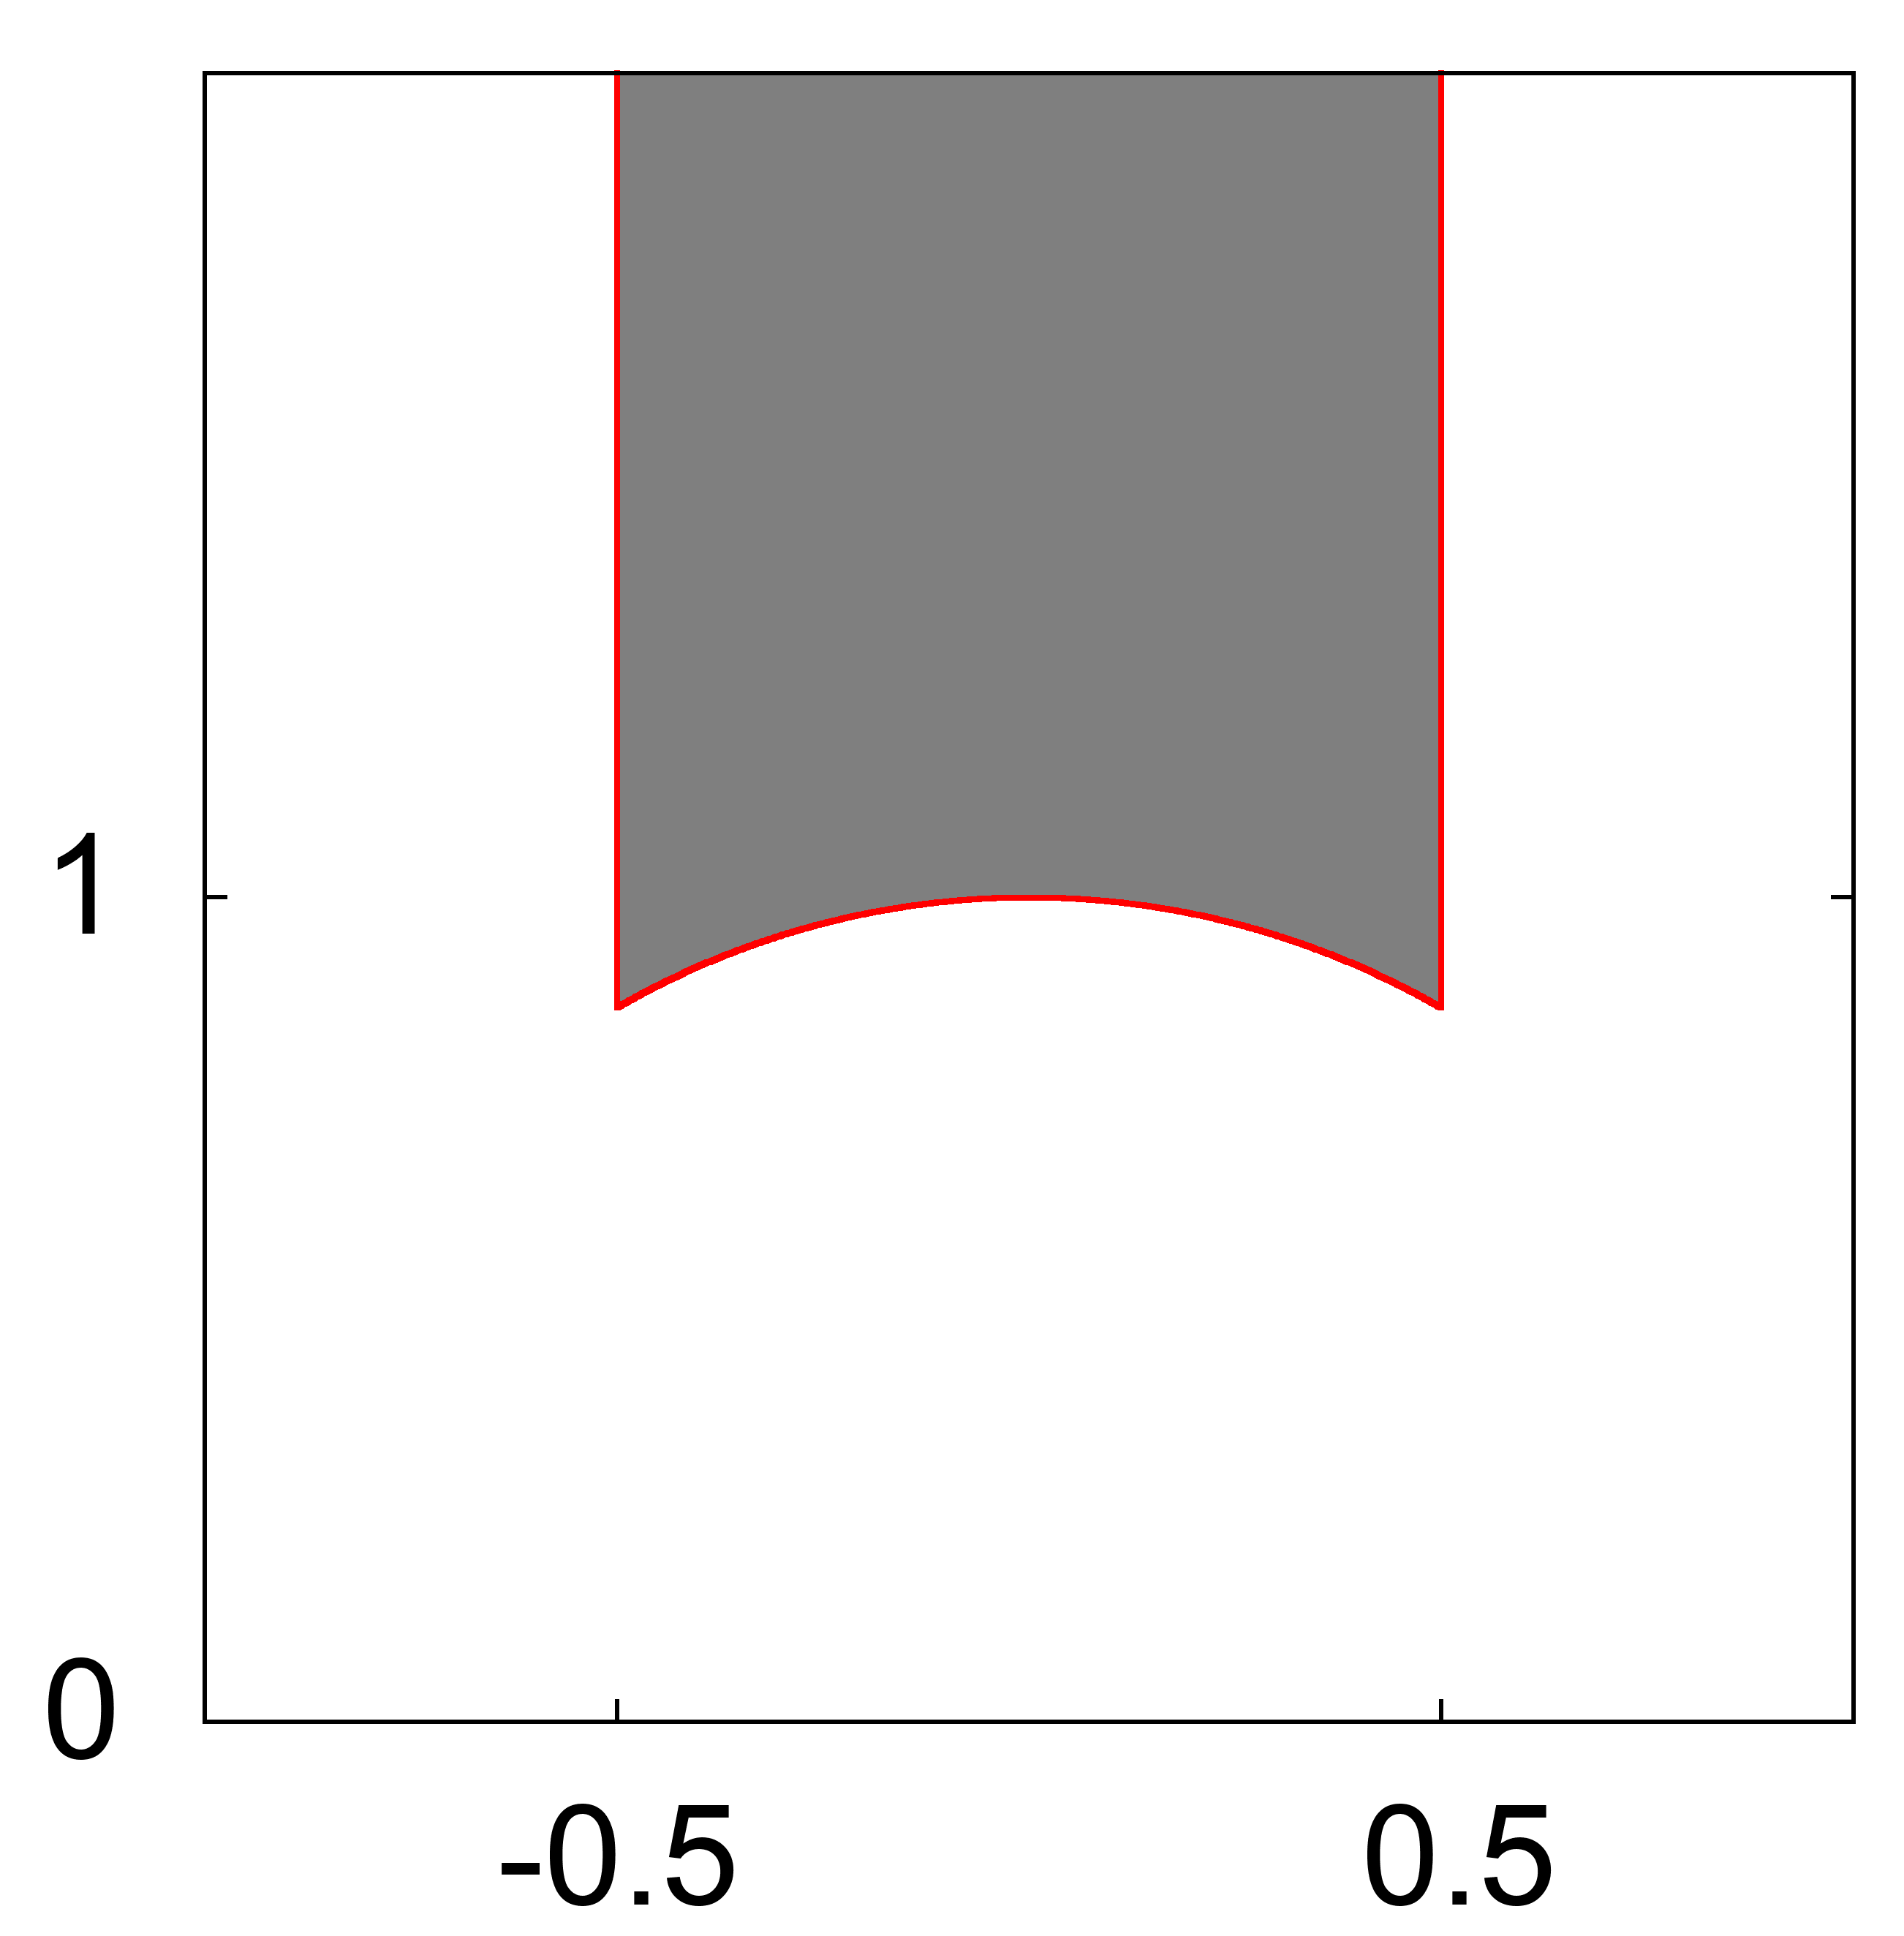
\includegraphics[width=3.5cm]{fd.png}
    \caption{Modular fundamental domain}
  \end{figure}

  We write $\tau = x+yi$ with $x,y\in\IR$ and $y>0$.
  Then $q=e^{-2\pi y} e^{2\pi x}$.
  If $\tau\in \cF$, then $|x|\le 1/2$ and $y\ge \sqrt{3}/2$.
  So $q$ as a function of $(x,y)$ is definable restricted to
  $\cF$. Moreover, $|q|\le e^{-\pi\sqrt{3}}< 1$. Now
  the $q$-expanion of $j$ restricted to the compact ball of radius
  $e^{-\pi\sqrt{3}}$ centered at $0$ is definable in $\IRan$.

  Putting things together we see that $j|_{\cF}\colon
  \cF\rightarrow\IC$ is definable in $\IRanexp$. The restriction is
  surjective.

  Let $m\in\IN$ and consider the product $(\tau_1,\ldots,\tau_m)\mapsto
  (j(\tau_1),\ldots,j(\tau_m))$ which we also denote by
  $j\colon\IH^m\rightarrow\IC^m$. We find that
  $j|_{\cF^m}\colon \cF^m\rightarrow\IC^m=Y(1)(\IC)$ is definable in $\IRanexp$.

  As in Example~\ref{ex:thetafunc} we can consider the preimage of an
  algebraic subvariety $V\subset Y(1)^m$ defined over $\IC$.
  Indeed,
  \begin{equation*}
    j^{-1}(V(\IC)) \cap \cF^m
  \end{equation*}
  is definable in $\IRanexp$ with $\dim j^{-1}(V(\IC))\cap \cF^m =
  2\dim V$.  
\end{example}

\section{Further Reading and Open Problems}

It is known that any function $f \colon \IR\rightarrow\IR$ that is
definable in $\IRan$ is polynomially bounded. That is, there exists
an integer $N\ge 1$ such that $|f(x)|\le x^N$ for all sufficiently
large $x$. This shows that $\exp$ is not definable in $\IRexp$. It is
also known that for any function $f\colon \IR\rightarrow\IR$ that is
definable in $\IRexp$ there exists an $N\ge 1$ such that $|f(x)| \le
\exp^{N}(x)$ for all sufficiently large $x$; here $\exp^{N}$ is the
$N$-fold iterated exponential function. 
Does there exist an o-minimal structure in which a function $f\colon
\IR\rightarrow\IR$ is definable and eventually grows faster than any
finite tower of exponentials?

Further reading:
\begin{itemize}
\item For an overview of o-minimal geometry we refer to the paper of
  van den Dries and Miller~\cite{DM:96}.

\item Theory of theta functions: Mumford's~\cite{MumfordTataLectures}.
\end{itemize}
% \begin{itemize}
% \end{itemize}

%%% Local Variables:
%%% TeX-master: "main"
%%% End:


%% Day 3, Wednesday, 60 minutes
\chapter{Functional Transcendence}

\section{Overview}

In this chapter we first state the Pila--Wilkie Theorem. This
important tool gives us information on the distribution of rational
points of bounded height on a definable set. We will see two
applications of this theorem. The first is towards some cases of the
Ax--Schanuel Theorem which is used to systematically treat situations
that arose in Section~\ref{subsub:functrans}. The second application
will come in a further chapter. 

\section{The Pila--Wilkie Theorem}


\begin{definition}
  Let $x\in \IQ$. There exist coprime integers $p,q$ with
  $q\ge 1$ and $x=p/q$. The (exponential) height of $x$ is $H(x)=\max\{|p|,q\}$.
  Let $(x_1,\ldots,x_m)\in\IQ^m$. % There exist coprime integers
  % $p_1,\ldots,p_m,q$ with $q\ge 1$ and $x_i = p_i/q$ for all $i\in
  % \{1,\ldots,m\}$.
  The exponential height of $(x_1,\ldots,x_m)$ is $H(x_1,\ldots,x_m)
  =\max \{H(x_1),\ldots,H(x_m)\}$. 
%  = \max_{1\le i\le m} \{|p_1|,\ldots,|p_m|,q\}$. 
\end{definition}

In Hector's lecture we will encouter heights that are normalized by
taking $\log H(\cdots)$ in the case $m=1$. In the context of the
Pila--Wilkie Theorem the exponential height is slightly more
practical.


\begin{example}\label{ex:heightcount1}\leavevmode
  \begin{enumerate}
  \item [(i)]
  One fundamental feature of the height is the Northcott property: for
  all $T\ge 1$ the set
  \begin{equation*}
    \{ x\in \IQ : H(x)\le T\}
  \end{equation*}
  is finite. In this statement we may replace $x\in\IQ$ by $x\in
  \IQ^m$.

  Let use define $a(T) = \#\{x\in\IQ : H(x)\le T\}$ which is
  non-decreasing in $T$. How quickly does $a(T)$ grow in $T$?
  If $T\ge 1$ is an integer, then $a(T) \ge 2T+1$ by considering
  integers
  $-T,-T+1,\ldots,0,\ldots,T-1,T$. But we have all rational numbers at
  our disposal and $H(x)=H(-x)=H(1/x)=H(-1/x)$ for all
  $x\in\IQ^\times$. So it suffices to count rational numbers in
  $(0,1)$ of height at most $T$, quadruple this number, and add 3
  (for $0,\pm 1$)
  ,\textit{i.e.}, 
  \begin{equation*}
    a(T) = 3 + 4 \sum_{q=1}^T \# \{ p : 1\le p \le q-1 \text{ and
    }\gcd(p,q)=1\} = -1+4\sum_{q=1}^T \varphi(q)
  \end{equation*}
  with $\varphi$ as in Section~\ref{sec:rootsof1}. By Lemma~\ref{lem:lgo}
  $a(T)$ grows at least as $T^{3/2}$. In fact, it is known that
  $a(T)\sim \frac{12}{\pi^2} T^2$ as $T\rightarrow\infty$.


\item[(ii)] Let $d\ge 1$ be an integer and consider
  $X = \{(x,x^d) : x\in \IR\}$. If $x\in\IQ$ then $H(x^d) = H(x)^d$.
  So
  \begin{equation*}
    \#\{ (x,y) \in X\cap \IQ^2 : H(x,y)\le T\} \sim
    \frac{12}{\pi^2}T^{2/d} 
  \end{equation*}
  as $T\rightarrow\infty$. 
  
  \item[(iii)] It follows from the Lindemann--Weierstrass Theorem that
    if $x\in\IQ^\times$, then $e^x \not\in\IQ$. So the graph
    $\{(x,e^x) : x\in\IR\}$ contains precisely $1$ rational point
    $(0,1)$.

  \item[(iv)] A transcendental graph can contain infinitely many
    rational points. Consider the graph of $x\mapsto 2^x$ on $\IR$, so 
    $X=\{(x,2^x) : x \in\IR\}$. This set is definable in $\IRexp$.
    If $t\ge 1$ is an integer and $x\in \{1,\ldots,t\}$, then
    $(x,2^x)$ is integral of height at most $T=2^t$. Therefore,
    \begin{equation*}
      \# \{(x,2^x)\in\IQ^2 : H(x,2^x)\le T\} \ge t= (\log T)/\log 2.
    \end{equation*}
    It is not difficult to prove an upper bound that is linear in
    $\log T$. 
\end{enumerate}
\end{example}

\begin{definition}
  Let $X\subset\IR^m$ be any subset and $T\ge 1$. The \emph{counting
    function} is 
  \begin{equation*}
    N(X,T) = \#\{ x\in X\cap \IQ^m : H(x)\le T\}. 
  \end{equation*}
\end{definition}

In our applications we will usually take $X$ to be a  set definable in
an o-minimal structure.

\begin{example}
  We revisit Example~\ref{ex:heightcount1} using the counting
  function.
  \begin{enumerate}
  \item [(i)] We have $N(\IR,T)\sim \frac{12}{\pi^2}T^2$ as
    $T\rightarrow\infty$.
  \item [(ii)] Let $d\ge 1$ be an integer and $X= \{(x,x^d):
    x\in\IR\}$. Then $N(X,T)\sim \frac{12}{\pi^2}T^{2/d}$ as
    $T\rightarrow\infty$.
  \item[(iii)] We have $N(\text{graph of }\exp,T) = 1$ for all $T\ge
    1$.
  \item [(iv)] We have $\log T \ll
    N(\text{graph of }x\mapsto 2^x,T)\ll \log T$ for $T\rightarrow\infty$.\footnote{$\ll$
      signifies that the left-hand side is bounded by a positive
      constant times the right-hand side.}
  \end{enumerate}
\end{example}


\section{Further Reading and Open Problems}

%%% Local Variables:
%%% TeX-master: "main"
%%% End:


%% Day 4, Thursday, 60 + 60 minutes, spill over to Friday?
\chapter{The Conjectures of Manin--Mumford and Andr\'e--Oort}

%%% Local Variables:
%%% TeX-master: "main"
%%% End:


%% Day 5, Friday, 60 + 60 minutes
\chapter{Unlikely Intersections}

%%% Local Variables:
%%% TeX-master: "main"
%%% End:


\bibliographystyle{alpha}
\bibliography{literature}

\vfill\hfill\texttt{\input{.git/refs/heads/master}}

\end{document}